\documentclass{article}
\usepackage{array}
\newcolumntype{P}[1]{>{\centering\arraybackslash}p{#1}}
\usepackage{float}

\usepackage{svg}
\usepackage[english]{babel}
% \usepackage{fontspec}
\usepackage{siunitx}
% \usepackage{microtype}
\usepackage{underscore} % Allows underscores in text and better handling
\usepackage[T1]{fontenc}
\usepackage{lineno,hyperref}
\usepackage[font=small,labelfont=bf]{caption}
\usepackage{subcaption}
\usepackage{mathtools}
\usepackage{booktabs}
\usepackage{tcolorbox}
\usepackage{enumerate}
\usepackage[inline]{enumitem}
\usepackage{amsmath}
\usepackage{svg}
\usepackage{listings}
\usepackage{appendix}
\usepackage{authblk} % for author and affiliation
\usepackage{longtable}
\usepackage{array}
\usepackage{makecell}
\usepackage{caption}

% Zio's formatting
\usepackage{setspace}
\usepackage{fancyhdr}
\usepackage{tikz}


\usepackage[
    backend=biber,
    style=numeric-comp,
    sorting=none,
    maxnames=8,
    minnames=3,
    maxcitenames=2,
    mincitenames=1,
    abbreviate=false,
    giveninits=true,
    date=year
]{biblatex}
\addbibresource{mybibfile.bib}
\providecommand{\keywords}[1]{\textbf{\textit{Keywords---}} #1}
% \renewcommand\Authfont{\normalsize\bfseries}
\renewcommand\Affilfont{\itshape\small}

\title{Enhanced Bayesian Network Model with Imprecise Probabilities for Concrete Degradation in Radioactive Waste Disposal due to Climate Change}

\author[1]{A.Perin}
\author[2]{S. A. Hosseini}
\author[2,3]{E. Zio}
\author[1]{M. Broggi}
\author[1,4,5]{M. Beer}

\affil[1]{Institute for Risk and Reliability, Leibniz Universität Hannover, Hannover 30167, Germany}
\affil[2]{Energy Department, Politecnico di Milano, Milan 20156, Italy}
\affil[3]{MINES Paris-PSL University, Centre de Recherche sur les Risques et les Crises (CRC), Sophia Antipolis, France}
\affil[4]{Department of Civil and Environmental Engineering, University of Liverpool, Liverpool L69 3GH, UK}
\affil[5]{International Joint Research Center for Resilient Infrastructure \& International Joint Research Center for Engineering Reliability and Stochastic Mechanics, Tongji University, Shanghai 200092, China}
% \author{A. Perin, S. A. Hosseini, E. Zio, M. Broggi, M. Beer}

\date{\today}

% Double line spacing from here on
\AtBeginDocument{\doublespacing}

\fancypagestyle{firstpagefooter}{
  \fancyhf{}
  \fancyfoot[L]{%
    \begin{tikzpicture}[remember picture, overlay]
      \node[anchor=south west, fill=gray!10, draw=black, rounded corners=2pt, inner sep=4pt]
      at ([xshift=1cm,yshift=1.5cm]current page.south west) {%
        \begin{tabular}{l}
            Name: Andrea Perin \\
            Date: \today \\
            Name: andrea.perin@irz.uni-hannover.de \\
        \end{tabular}
      };
    \end{tikzpicture}
  }
  \renewcommand{\headrulewidth}{0pt}
  \renewcommand{\footrulewidth}{0pt}
}

\begin{document}

\maketitle
\thispagestyle{firstpagefooter}

\begin{abstract}\label{abstract}
    %chktex-file 46
The susceptibility of concrete structures to chemical corrosion is significantly influenced by environmental exposure, a condition intensified by climate change. 
Bayesian Network has demonstrated significant effectiveness in modeling the interdependencies in such corrosion processes. However, traditional Bayesian Networks face challenges in addressing aleatoric and epistemic uncertainties and in accommodating the impacts induced by climate change on corrosion dynamics. We propose an enhanced Bayesian Network framework that aims to effectively manage these uncertainties by leveraging continuous nodes and incorporating imprecise probabilities, especially from climate change projections. This framework is applied to carbonation and chloride corrosion phenomena, which are the main degradation mechanisms in concrete structures, considering the intertwined uncertainties associated with environmental parameters such as temperature, $CO_2$ concentration, and relative humidity over time. The results demonstrate the significant capabilities of the enhanced Bayesian Network framework, not only by improving structural safety analysis to disentangle from the remaining uncertainties but also by advancing the mitigation strategies for corrosion risks in concrete structures.

\end{abstract}
\keywords{radioactive waste disposal, concrete structure, chemical corrosion, climate change, structural reliability analysis, risk assessment, enhanced Bayesian networks, imprecise probability}

\section{Introduction}\label{introduction}
    %chktex-file 46
%chktex-file 9
%chktex-file 10

Concrete is a fundamental material for buildings, bridges, tunnels and other structures with safety-critical containment functions like those employed in nuclear power plants and radioactive waste disposals.
This is because of its proven strength, durability and cost-effectiveness.
However, environmental exposure can accelerate its degradation~\cite{GLASSER2008226}. For example, structures located in coastal or urban areas, where humidity, chlorides and fluctuating temperatures accelerate deterioration, are especially prone to corrosion-related processes~\cite{qu2021durability}.
One such process is carbonation, where atmospheric carbon dioxide ($CO_2$) reacts with calcium compounds by forming calcium carbonate, challenging the reinforced concrete structures through the reduction of the alkalinity of the concrete, that is, lowering the PH, which compromises the protective layer surrounding the embedded steel reinforcement.
As carbonation progresses and pH decreases, this protective layer breaks down, leaving steel vulnerable to corrosion~\cite{carbonation}.
This degradation can lead to cracks, cracking, and weakening of the bond between the steel and concrete, ultimately diminishing the structural durability.
Another degradation mechanism is chloride-induced corrosion, which leads to the accumulation of chloride ions around the embedded steel reinforcement. Unlike carbonation, chloride ions can penetrate even high-alkalinity concrete without necessarily lowering the pH, directly compromising the passive film on steel.
Once a critical chloride concentration threshold is reached on the steel surface, localized corrosion begins, often in the form of pitting~\cite{shi2012durability}.
The process of corrosion of concrete structures must be taken into account for safety-critical applications on long-term periods, like for the containment barriers of radioactive waste repositories~\cite{walton1990models}.
To maintain structural integrity over such long service lifes, the risk assessment must consider the environmental stress uncertainties, as they evolve over the long time horizons~\cite{lindborg2018climate}.
\\

Traditional risk assessment tools, such as Event Trees (ET)~\cite{papazoglou_mathematical_1998} and Fault Trees (FT)~\cite{kabir_overview_2017}, are the most widely used for the risk assessment of nuclear power plants and radioactive waste disposals.
However, they are inherently limited by Boolean logic and the treatment of dependencies.
Bayesian Networks (BNs), which model system dependencies through directed acyclic graphs~\cite{mahadevan2001bayesian} can also account for the uncertainties due to imperfect knowledge on system behaviour, include common cause failures and consider multistate events. \\
A BN enables diagnostic problem-solving while preserving the multi-scenario analysis and minimal cut-set identification features inherent to FT analysis.
Since risk assessment often involves conditional probabilities, BNs provide an efficient factorization of joint probability distributions, making them particularly useful for reliability analysis, for example as shown by the work of~\textcite{langseth_bayesian_2007}.
BNs have been used in several applications, including maintenance planning of structural components~\cite{morato2022optimal}, multi-hazard fragility assessment of bridges~\cite{gehl2016development, barros2024gaussian}, disaggregation of structural failure~\cite{yazdani2020bayesian}, deterioration processes in engineering structures~\cite{luque2019risk,lee2023dynamic,tran2020dynamic}, and especially reliability assessment of reinforced concrete structures~\cite{hackl2016reliability,hosseini2024dynamic,guo2024mixed}.\\
Despite their advantages, conventional BNs are limited in their ability to model aleatoric uncertainties, as they primarily rely on expert knowledge and discrete probability assignments.
Given that the uncertainties in corrosion dynamics are strongly influenced by $CO_2$ concentration, temperature and relative humidity, it is important to incorporate climate change projections in the modelling.\\
In this paper, we propose an enhanced Bayesian Network (eBN) with the incorporation of imprecise probabilities for handling both aleatoric and epistemic uncertainties.
The eBN framework integrates structural reliability methods, such as First-Order Reliability Methods (FORM), and advanced Monte Carlo techniques into conventional BN structures. 
The extension allows eBNs to: 
\begin{enumerate*}[label=\roman*)]
  \item incorporate aleatoric uncertainties by introducing continuous nodes associated with probability distributions, significantly enhancing their applicability to risk assessment;
  \item combine the probabilistic reasoning capabilities with well-established reliability methods;
  \item adopt imprecise probabilities into the eBN framework, incorporating both epistemic and aleatoric uncertainties into the assessment process;
  \item model complex interactions between environmental variables and material properties over time.
\end{enumerate*} 
Thus, the eBN framework enables the embedding of climate change projections variables, e.g., $CO_2$ concentrations, temperature and humidity, into the corrosion process and allows a scenario-based evaluation of the impact of the environmental conditions over the chemical degradation of concrete in time.
With the ability to assess climate change scenarios, eBNs offer an innovative framework, enabling the assessment of the resilience of concrete structures in the face of evolving environmental stressors, ultimately enabling risk-informed decision-making for adaptation and mitigation strategies.\\

The proposed eBN modelling framework is applied to the near-surface radioactive waste disposal located in Dessel, Belgium~\cite{tosoni_comprehensiveness_2019-1}.
Three climate change scenarios are considered, each corresponding to a distinct Shared Socioeconomic Pathway (\textit{ssp}) relevant to the region~\cite{CMIP6}.
These projections are used to extrapolate the temporal evolution that influences the distribution of relevant parameters involved in carbonation-induced and chloride-induced corrosion processes.
The primary objectives of this study are to: 
\begin{enumerate*}[label=\roman*)]
    \item develop an eBN modelling framework tailored to the Dessel disposal that accounts for aleatoric uncertainties affecting structural integrity;
    \item quantify the impact of epistemic uncertainty associated with climate change projections; and
    \item support informed decision-making through a multi-scenario risk assessment.
\end{enumerate*}
\\

The remaining sections of the manuscript are structured as follows: Section~\ref{ebn} formulates the eBN-based framework with incorporation of imprecise probabilities; Section~\ref{caseofstudy} describes the case study regarding two relevant degradation processes, carbonation-induced and chloride-induced corrosions, affecting concerete structures related to radioactive waste disposals; and Section~\ref{results} presents the results. In Section~\ref{conclusions}, conclusions are drawn.

% Risk assessment plays a pivotal role in ensuring the safety and reliability of complex engineering systems, particularly in safety-critical domains such as aerospace, nuclear power, and offshore industries.
% The increasing complexity of these systems necessitates robust methodologies to prevent design and operational failures, optimize safety criteria, and avoid excessive conservatism in risk evaluations.
% A well-structured risk assessment process is essential for guiding decision-making and preventing catastrophic events, as illustrated by past disasters such as the Piper Alpha offshore oil explosion~\cite{Piper_alpha}, the Seveso industrial accident~\cite{Seveso}, and the Clapham Junction rail crash!\cite{Clapham}. \\
% To be effective, a risk assessment framework must be both accurate and comprehensive, capable of accounting for multiple failure scenarios, uncertainties, and the varying quality of available information. Moreover, the framework should support decision-making in a computationally efficient manner, balancing precision with feasibility. \\
% Traditional risk assessment tools, such as Event Trees (ET)~\cite{papazoglou_mathematical_1998} and Fault Trees (FT)~\cite{kabir_overview_2017}, are the most widely used for prognosis analysis but are inherently limited by Boolean logic, making them unsuitable for an exhaustive dependability analysis. Bayesian Networks (BNs), which model system dependencies through directed acyclic graphs, can be seen as generalized FTs. BNs framework can model uncertainties in the behavior of the \textit{and} and \textit{or} gates, express imperfect knowledge on system behavior by incorporating Common Cause Failures and consider multi-state events, by including probabilistic dependencies. Furthermore, a BN enables diagnostic problem-solving while preserving the multi-scenario analysis and minimal cut-set identification features inherent to FT analysis.
% Since risk assessment often involves conditional probabilities, BNs provide an efficient factorization of joint probability distributions, making them particularly useful for reliability analysis as shown by the work of~\textcite{langseth_bayesian_2007}. \\
% Despite their advantages, traditional BNs are limited in their ability to model aleatoric uncertainties, as they primarily rely on expert knowledge and discrete probability assignments.\\

% \subsection{Concrete structures}
% Concrete is one of the most fundamental materials in modern infrastructure, forming the backbone of buildings, bridges, tunnels, and various critical structures.
% Its widespread use is due to its strength, durability, and cost-effectiveness.
% Beyond its mechanical properties, concrete interacts with the environment over time, undergoing chemical processes that influence both its performance and sustainability. 
% One such process is carbonation, where atmospheric carbon dioxide ($CO₂$) reacts with calcium compounds in hardened concrete, forming calcium carbonate.
% This natural reaction allows concrete to absorb CO₂ throughout its lifespan, contributing to carbon sequestration and reducing its overall environmental footprint. While carbonation provides potential environmental benefits, it also presents challenges for reinforced concrete structures. One of the primary concerns is the reduction of concrete’s alkalinity, which compromises the protective layer surrounding embedded steel reinforcement. In fresh concrete, the highly alkaline environment naturally forms a passive film on the steel, preventing it from corroding.
% However, as carbonation progresses and the pH decreases, this protective layer breaks down, leaving the steel vulnerable to corrosion~\cite{carbonation}.
% This deterioration can lead to cracks, spalling, and weakening of the bond between the steel and concrete, ultimately diminishing the structural capacity of the system. Given the widespread use of reinforced concrete in critical infrastructure, it is essential to account for corrosion risks to ensure long-term reliability and safety. \\
% Assessing the risk of corrosion in concrete structures is particularly important in safety-sensitive applications such as radiocative waste repositories. The extent of degradation depends on factors such as environmental exposure, material composition, and design considerations. Structures located in coastal or urban areas, where humidity, chlorides, and fluctuating temperatures accelerate deterioration, are especially prone to corrosion-related failures. To maintain structural integrity and extend service life, risk assessment frameworks must incorporate these environmental and material factors, allowing for the development of predictive models and preventive maintenance strategies. \\
% Failing to account for corrosion in the risk assessment of concrete structures can lead to severe safety risks and significant financial consequences. Historical failures, such as bridge collapses and the deterioration of aging nuclear containment facilities, emphasize the necessity of evaluating long-term structural durability. However, traditional risk assessment methods often rely on current environmental conditions without fully considering the evolving impact of climate change. Given that carbonation and corrosion rates are strongly influenced by CO₂ concentration, temperature, and relative humidity, it is essential to incorporate climate change projections into risk analysis tools to ensure more accurate assessments of structural longevity.
% Rising atmospheric CO₂ levels can accelerate the carbonation process, reducing the alkalinity of concrete at a faster rate and compromising the passive protection of embedded steel. Similarly, increasing global temperatures can enhance the diffusion of carbon dioxide into concrete, further amplifying carbonation effects. At the same time, shifts in relative humidity play a critical role in corrosion dynamics. Higher humidity levels promote corrosion once carbonation has reached the reinforcement, while excessively dry conditions can slow carbonation. These interdependent factors suggest that static, present-day environmental assumptions may underestimate long-term structural degradation risks. \\

% \subsection{Proposed solution}
% To address this, it is crucial to integrate probabilistic modeling approaches that incorporate climate projections, allowing for scenario-based evaluations of how changing environmental conditions will impact the deterioration of reinforced concrete over time. By employing models that account for uncertainty in climate variables, engineers can develop more adaptive and forward-looking maintenance strategies, ensuring the resilience of infrastructure in the face of evolving environmental stressors. 
% A comprehensive risk assessment framework must therefore move beyond conventional methodologies and embrace an uncertainty-aware approach that integrates climate science, probabilistic modeling, and structural reliability analysis. \\
% The proposed solution to address the limitations of traditional BNs regarding aletoric uncertainties and the need of tool capable to deal with epistemic uncertainties is the Enhanced Bayesian Network (eBN) with imprecise probabilities.
% The eBN framework integrates structural reliability methods—such as Monte Carlo simulation, First-Order Reliability Methods (FORM), and Advanced Monte Carlo techniques—into traditional BN structures. This extension allows eBNs to incorporate aleatoric uncertainties by introducing continuous nodes associated with probability distributions, significantly enhancing their applicability to risk assessment. By combining the probabilistic reasoning capabilities of BNs with well-established reliability methods, eBNs provide a powerful and flexible tool for assessing risks in engineering systems, ultimately improving decision-making processes and system safety.\\
% Introduction of imprecise probabilities into the eBN framework addresses the problem of a reliable risk assessment. By incorporating both epistemic uncertainties into the assessment process. The eBNs with imprecise probabilities provide a robust and flexible framework capable of modeling the complex interactions between environmental variables and material properties over time. This approach enables the incorporation of climate projections—such as CO₂ concentrations, temperature, and humidity—into risk models, facilitating a more comprehensive understanding of how these factors influence the long-term durability of concrete structures. With the ability to assess multiple failure scenarios under changing environmental conditions, eBNs offer a forward-thinking tool that enhances the predictive power and reliability of risk assessments, ultimately enabling better-informed decision-making regarding maintenance, repair, and mitigation strategies.


\section{eBN-based Modelling Framework}\label{ebn}
    %chktex-file 46

EBN is a directed acyclic graph designed to improve traditional BN modeling by incorporating both discrete and continuous events for a more comprehensive probabilistic analysis.
Both eBNs and BNs frameworks consist of two primary elements: nodes and edges. A node represents an event with its possible outcomes whose proability of occurrence are defined through a Conditional Probability Table (CPT); an edge expresses a direct dependence among two nodes, where the originating node is termed the parent and the arrival node is called the child.
A node with no incoming edges is referred to as a root node. 
% Nodes that are directly connected by outgoing edges from a given node are called its child nodes.
Non-root nodes have a CPT determined by the combination of the probabilities of all their discrete parents' states.\\

\subsection{eBN main features}
In a traditional BN, each node represents a discrete random variable that can take on a finite number of mutually exclusive and collectively exhaustive states.
For instance, root nodes \textit{A} and  \textit{B}, as well as node \textit{D} in the network depicted in Fig.~\ref{1_ebn_example}, fall into this category.
These nodes are referred to as discrete nodes, and their CPTs are defined using precise probability values, as illustrated in Table~\ref{1_example_CPTs}.
The traditional BN framework is extensively discussed in the work of \textcite{russell_computer}, and its application to reliability analysis is examined in detail in the study by \textcite{langseth_bayesian_2007}.
% These methodologies have been widely adopted in various domains, including risk assessment and decision-making under uncertainty. \\
The eBN framework here proposed is capable of handling continuous nodes, which are nodes associated with continuous random variables and, consequently, an infinite number of possible states.
The CPT of such nodes is defined using a probability density function (PDF) when the node is a root node, and using a conditional PDF when the node has one or more discrete parents.
For instance, node \textit{C} in Fig.~\ref{1_ebn_example} has a CPT characterized by a univariate normal distribution, $Normal(0,1)$, as illustrated in Table~\ref{1_example_CPTs}. \\  
A node whose CPT is not explicitly defined a priori but instead determined through a model that maps the inputs from its parent nodes to an output generated by the model itself, is referred to as a functional node.
The functional nodes can be continuous or discrete. 
In the case of continuous functional nodes, the model alone is sufficient to empirically reconstruct the corresponding CPT.\ 
However for discrete functional nodes, a performance function is required to define their two possible states, which typically represent a failure state and a safe state.
For example, node \textit{M} in Fig.~\ref{1_ebn_example} is a discrete functional node that operates based on this performance function. \\

\begin{figure}[h]
    \centering
    \begin{subfigure}{0.45\textwidth}
        \centering
        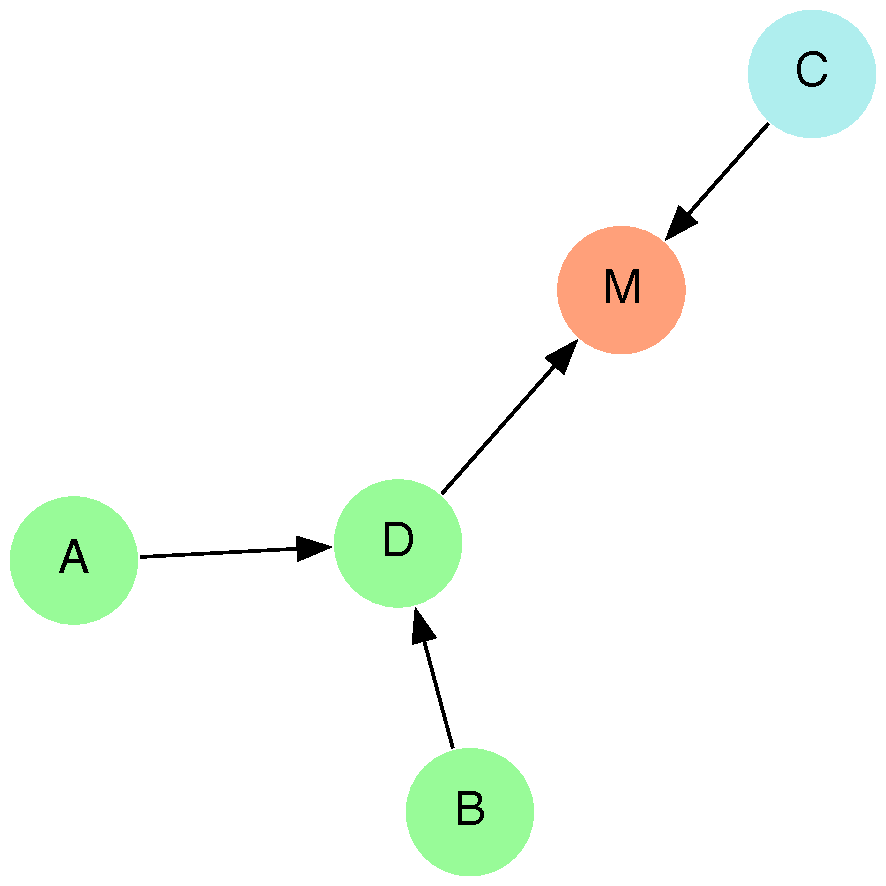
\includegraphics[width=\linewidth]{imgs/pdfs/1_ebn.pdf}
        \caption{Example of an eBN with two discrete root nodes \textit{A} and \textit{B}, one continuous root node \textit{C}, one discrete non-root node \textit{D} and one discrete functional node \textit{M}}\label{1_ebn_example}
    \end{subfigure}
    \hfill
    \begin{subfigure}{0.45\textwidth}
        \centering
        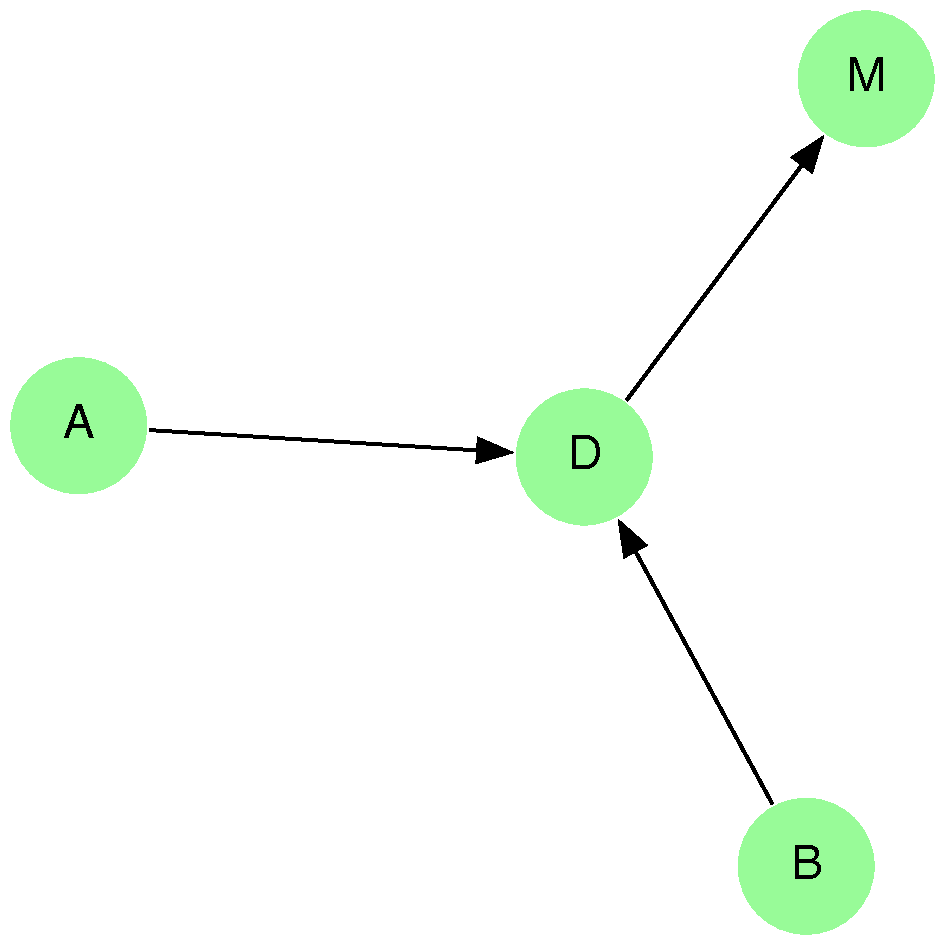
\includegraphics[width=\linewidth]{imgs/pdfs/2_rbn.pdf}
        \caption{Associated rBN where the continuous node \textit{C} is eliminated and the functional node \textit{M} is evaluated}\label{1_rbn_example}
    \end{subfigure}
    \caption{Example of reduction of an eBN when no continuous node is discretized}\label{1_reduction_no_disc}
\end{figure}

\begin{table}[!ht]
    \begin{center}
    \caption{CPTs of the eBN}\label{1_example_CPTs}
        \begin{tabular}{P{1.2cm}P{3.9cm}}
            \toprule
            \textbf{Node} & \textbf{CPT} \\
            \midrule
            A & 
                \begin{tabular}{p{0.5cm}p{0.5cm}}
                    \:a1 & \:a2 \\
                    \midrule $0.5$ & $0.5$\\
                \end{tabular}
                \\
                \midrule
            B & 
            \begin{tabular}{p{0.5cm}p{0.5cm}}
                \:b1 & \:b2 \\
                \midrule $0.3$ & $0.7$\\
            \end{tabular}
            \\
            \midrule
            C & $Normal(0;1)$
            \\
            \midrule
            D & 
                \begin{tabular}{p{1.6cm}p{0.5cm}p{0.5cm}}
                    \textbf{scenario} & \:d1 & \:d2 \\
                    \midrule
                    \:a1 \:b1 & $0.6$ & $0.4$ \\
                    \:a1 \:b2 & $0.1$ & $0.9$ \\
                    \:a2 \:b1 & $0.5$ & $0.5$ \\
                    \:a2 \:b2 & $0.5$ & $0.5$ \\
                \end{tabular}
            \\
            \midrule
            M & \begin{tabular}{p{3.3cm}}
                    M:\ $f(d,c) = d - c$ \\
                    P:\ $1-f(d,c) < 0$\\
                \end{tabular}
                \\
        \end{tabular}
    \end{center}
\end{table}

The eBN framework retains the core advantages of traditional BNs, such as the ability to perform multi-scenario analysis, serving as a multidisciplinary aggregator of information, and providing a clear visual representation of complex problems through structured parent-child relationships. 
eBNs further enhance modelling capabilities by incorporating aleatoric uncertainties through the inclusion of continuous nodes.
This addition allows for a more robust and realistic representation of uncertain phenomena, thereby improving the model's ability to reflect real-world complexities.\\

Let $\mathbf{Y} = \{Y_1, \ldots, Y_{n_Y}\}$ represent the collection of discrete nodes in the eBN, where each $Y_i$ is a discrete random variable with $k_i$ possible states $\{y_i^1, \ldots, y_i^{k_i}\}$, and let $\mathbf{X} = \{\mathbf{X}_1, \ldots, \mathbf{X}_{n_X}\}$ denote the collection of continuous nodes, where each $\mathbf{X}_i$ is associated with a set of continuous random variables, $\mathbf{X}_i = \{X_{i,1}, \ldots, X_{i,n_i}\}$. The joint distribution function of the system can, then, be expressed through the factorization given in Eq.~\ref{2:factorization_ebn}; this mathematical formulation, combined with the application of structural reliability methods (SRMs) to compute joint probability measures in networks with continuous parents, is detailed in the work of \textcite{straub_bayesian_2010}:

\begin{equation}
    \label{2:factorization_ebn}
    p(\mathbf{y}|\mathbf{x})f(\mathbf{x}) = \prod_{Y_i\in \mathbf{Y}} p(y_i|Pa(Y_i)) \prod_{X_i\in \mathbf{X}} f(\mathbf{x}_i|Pa(\mathbf{X}_i)) 
\end{equation}

One of the key strengths of BNs is their ability to utilize exact algorithms to perform \textit{inference} based on available \textit{evidence}, meaning the system's probabilities can be updated given any observed value of a node within the network.
This feature enables BNs to provide accurate and efficient reasoning about uncertain systems. 
% However, in the case of the eBN framework, the application of exact-inference algorithms is not directly feasible due to the inclusion of continuous nodes.
The continuous nature of these nodes complicates the inference process, as they introduce infinite possible states, making traditional exact-inference algorithms inapplicable.  
To address this limitation, once the CPTs for all functional nodes are evaluated, a \textit{node elimination} algorithm, derived from graph theory~\cite{Shachter86a}, is employed. 
This algorithm systematically removes the continuous nodes from the network while preserving the acyclicity of the eBN at each step,  transforming the network into its reduced form (rBN), as illustrated in Fig.~\ref{1_reduction_no_disc}. 
By applying this algorithm, the eBN is reduced to a standard BN, which is referred to as the \textit{reduced} BN.\ This reduction allows for the use of well-established exact-inference algorithms for BNs, which enable both prognostic and diagnostic analysis. \\

\begin{figure}[h]
    \centering
    \begin{subfigure}{0.45\textwidth}
        \centering
        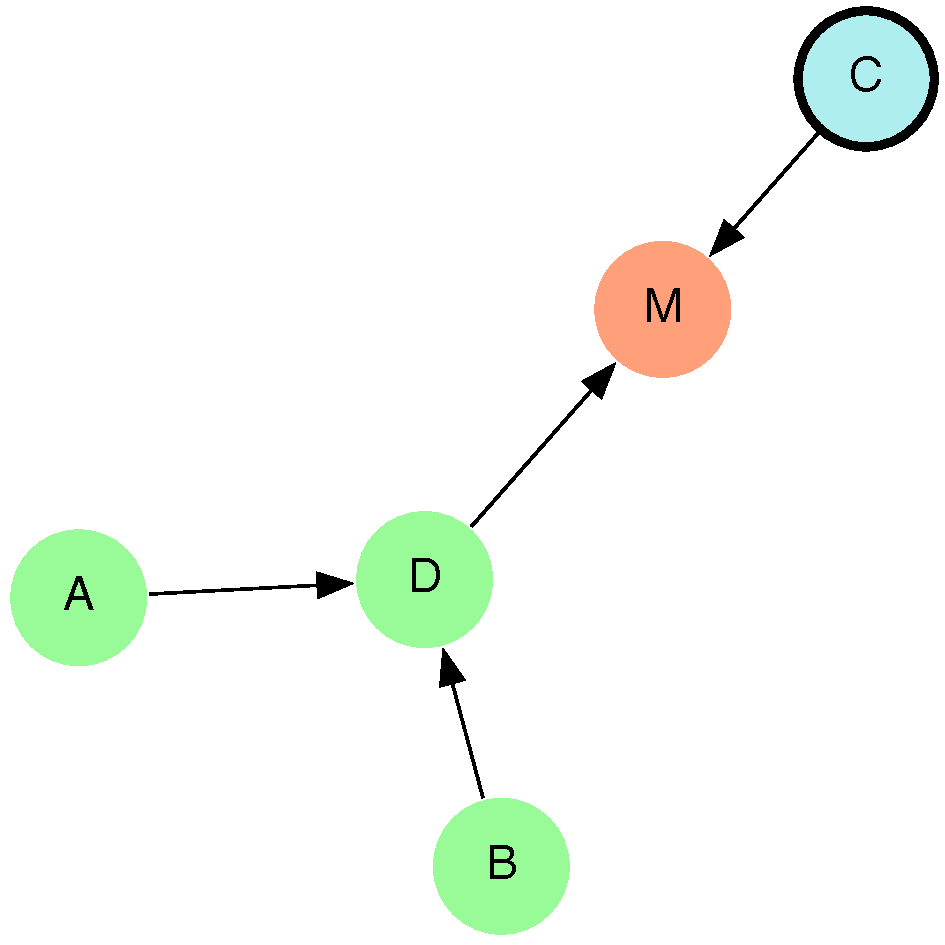
\includegraphics[width=\linewidth]{imgs/pdfs/3_d_ebn.pdf}
        \caption{Example of the same eBN of Fig.\ref{1_ebn_example} with continuous node \textit{C} to be discretized}\label{1_ebn_disc_example}
    \end{subfigure}
    \hfill
    \begin{subfigure}{0.45\textwidth}
        \centering
        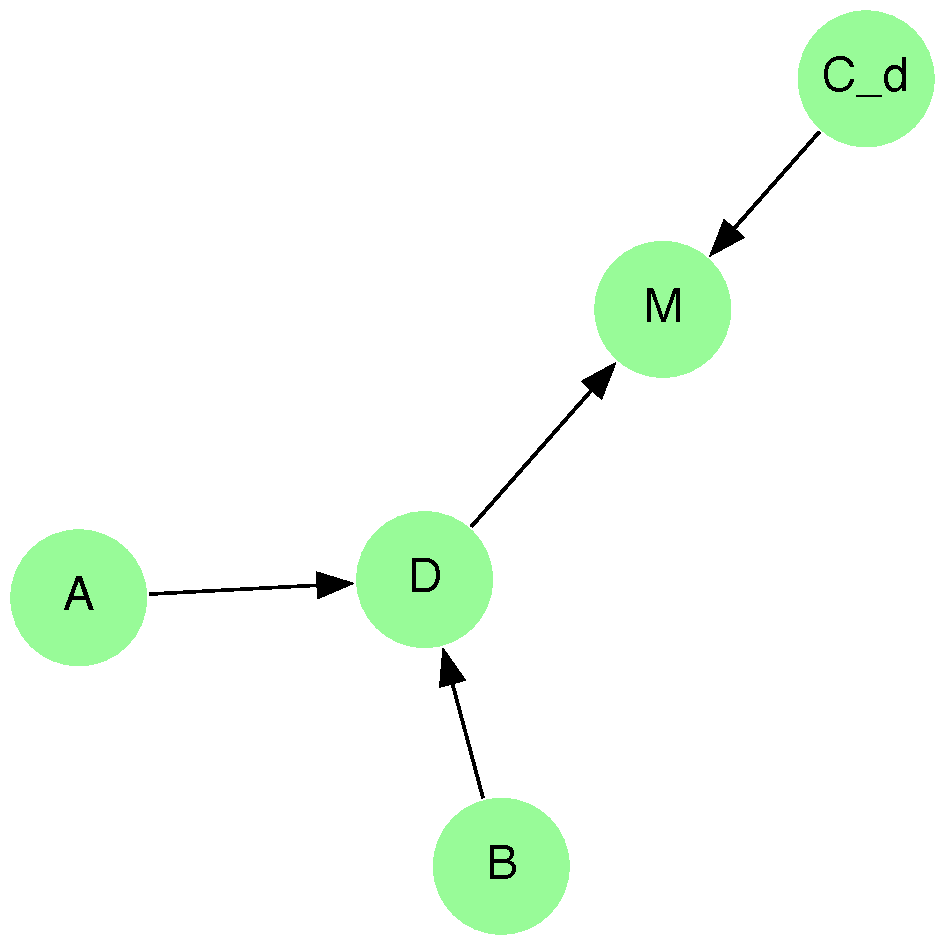
\includegraphics[width=\linewidth]{imgs/pdfs/4_d_rbn.pdf}
        \caption{Associated rBN where the continuous node \textit{C} is discretized into \textit{Cd}}\label{1_rbn_disc_example}
    \end{subfigure}
    \caption{Example of reduction of an eBN when a continuous node is discretized}\label{1_reduction_disc}
\end{figure}

\begin{table}[hbt!]
    \begin{center}
        \caption{CPT of the discretized node \textit{Cd} with a $[-3;0;3]$ discretization interval}\label{exact_disc_tab}
        \begin{tabular}{P{1.5cm}P{1.5cm}P{1.5cm}P{1.5cm}}
            \textbf{$[-\infty;-3]$} & \textbf{$[-3;0]$} & \textbf{$[0;3]$} & \textbf{$[3;\infty]$} \\
            \midrule
            $0.0013499$ & $ 0.49865$ & $ 0.49865$ & $0.0013499$ \\
        \end{tabular}
    \end{center}
\end{table}

\begin{table}[hbt!]
    \begin{center}
        \caption{CPT of the node \textit{M} after being evaluated}\label{Mnode_tab}
        \begin{tabular}{P{2cm}P{2cm}P{2cm}}
            \textbf{scenarios} & \textbf{$M fail$} & \textbf{$M safe$} \\
            \midrule
            $d1;[-\infty;-3]$ & $0$ & $1$ \\
            $d1;[-3;0]$ & $0$ & $1$ \\
            $d1;[0;3]$ & $ 0.48$ & $0.52$ \\
            $d1;[3;+\infty]$ & $ 1$ & $0$ \\
            $d2;[-\infty;-3]$ & $0$ & $1$ \\
            $d2;[-3;0]$ & $0$ & $1$ \\
            $d2;[0;3]$ & $0.79$ & $0.21$ \\
            $d2;[3;+\infty]$ & $1$ & $0$ \\
        \end{tabular}
    \end{center}
\end{table}

Once all continuous nodes have been removed from the network during the network reduction phase, both exact and approximated discretization algorithms can be employed to either consider evidence over these nodes or update their CPTs.
This is shown in Fig.~\ref{1_reduction_disc} where the continuous node \textit{C} is discretized into the discrete node \textit{Cd} with the corresponding CPT shown in Tab.~\ref{exact_disc_tab}. 
By discretizing the continuous nodes, it becomes possible to incorporate them into the inference process, allowing for the evaluation of conditional probabilities that involve the former continuous nodes. 
This is illustrated in Tab.~\ref{direct_inference_tab} for the direct inference problem and in Tab.~\ref{inverse_inference_tab} for the inverse inference problem.
The discretization algorithm allows effectively integrating continuous nodes into the eBN framework, enabling the use of traditional inference techniques while accurately representing aleatoric uncertainty as continuous random variables.\\
Therefore, eBN integrates classical probabilistic modelling with structural reliability methods to form a robust framework for both prognosis and diagnosis across various engineering domains, enhancing decision-making through a more accurate and realistic representation of uncertainty associated with continuous variables. 
% The discretization process ensures that aleatoric uncertainty is effectively captured while preserving the generality of the inference process.\\

\begin{table}[hbt!]
    \begin{center}
        \caption{Direct inference results on node \textit{M} given node $Cd$ state}\label{direct_inference_tab}
        \begin{tabular}{P{3cm}P{3cm}P{3cm}}
            \textbf{evidence} & \textbf{$P(M=fail | Cd)$} & \textbf{$P(M=safe | Cd)$} \\
            \midrule
            $Cd = [-\infty;-3]$ & $0$ & $1$  \\
            $Cd = [-3;0]$ & $0$ & $1$  \\
            $Cd = [0;3]$ & $0.99605$ & $0.00395$ \\
            $Cd = [3;\infty]$ & $0.00395$ & $0.99605$\\
        \end{tabular}
    \end{center}
\end{table}

\begin{table}[hbt!]
    \begin{center}
        \caption{Inverse inference results on node $Cd$ given node \textit{M} in a failure state}\label{inverse_inference_tab}
        \begin{tabular}{P{3cm}P{4cm}}
            \textbf{Query} & \textbf{$P(Query | M = M fail)$} \\
            \midrule
            $Cd = [-\infty;-3]$ & $0$ \\
            $Cd = [-3;0]$ & $0$ \\
            $Cd = [0;3]$ & $0.68305$ \\
            $Cd = [3;\infty]$ & $1$ \\
        \end{tabular}
    \end{center}
\end{table}

\subsection{Imprecise probabilities}
In the current eBN framework, only aleatoric uncertainties are explicitly considered, represented by univariate PDFs, whereas discrete nodes are assigned crisp probability values. 
However, in real-world applications, both probability distributions and probability assignments often rely on subjective expert judgments and possibly only incomplete or limited data. 
This reliance on subjective probabilities arises from different factors, such as the inherent impossibility to estimate some system parameters and the difficulty in obtaining relevant informative data. 
To address this challenge, imprecise probability theory provides a robust and flexible mathematical framework~\cite{beer_imprecise_2013-1} for modelling epistemic uncertainties. 
These uncertainties stem from sources such as conflicting expert opinions, sparse or incomplete datasets, measurement errors and general knowledge gaps that are common in many engineering and decision-making contexts. 
An eBN that incorporates imprecise probabilities will be referred to as an imprecise eBN throughout the remainder of this paper, enabling more accurate representations of uncertainty in complex systems.

\begin{figure}[h]
    \centering
    \begin{subfigure}{0.45\textwidth}
        \centering
        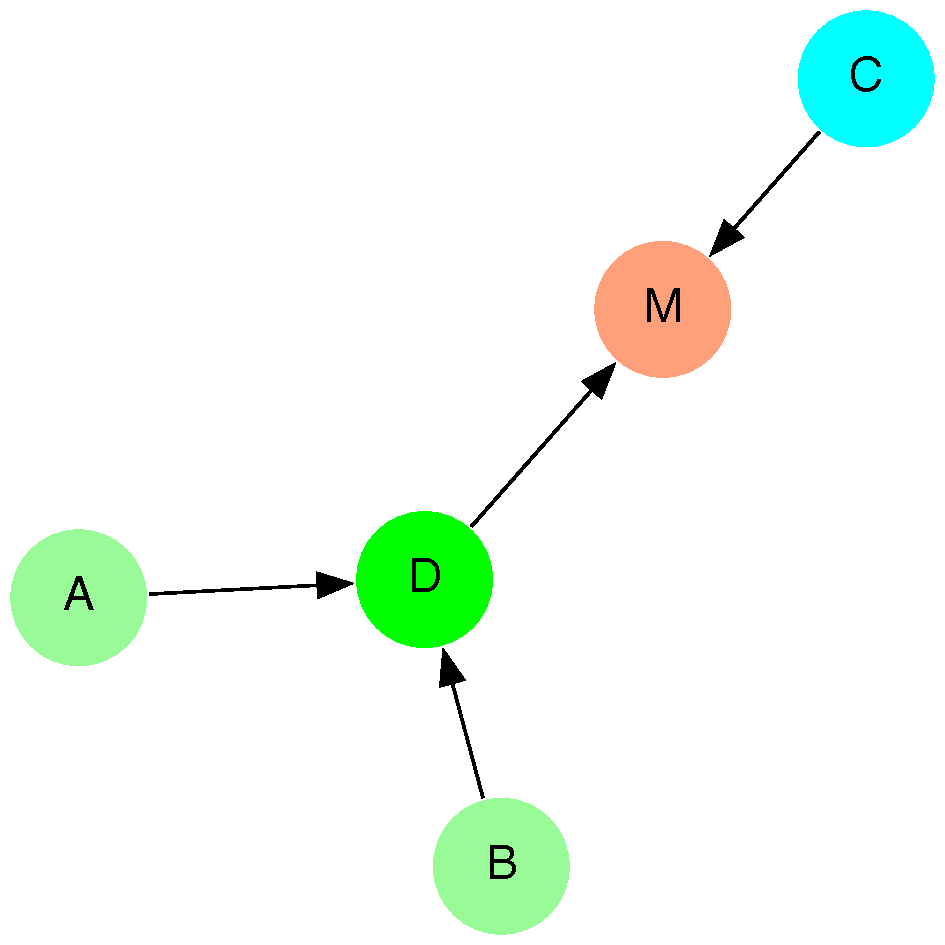
\includegraphics[width=\linewidth]{imgs/pdfs/5_imprecise_ebn.pdf}
        \caption{Example of the same eBN of Fig.\ref{1_ebn_example} but continuous node \textit{C} and discrete node \textit{D} are imprecise}\label{1_imp_ebn}
    \end{subfigure}
    \hfill
    \begin{subfigure}{0.45\textwidth}
        \centering
        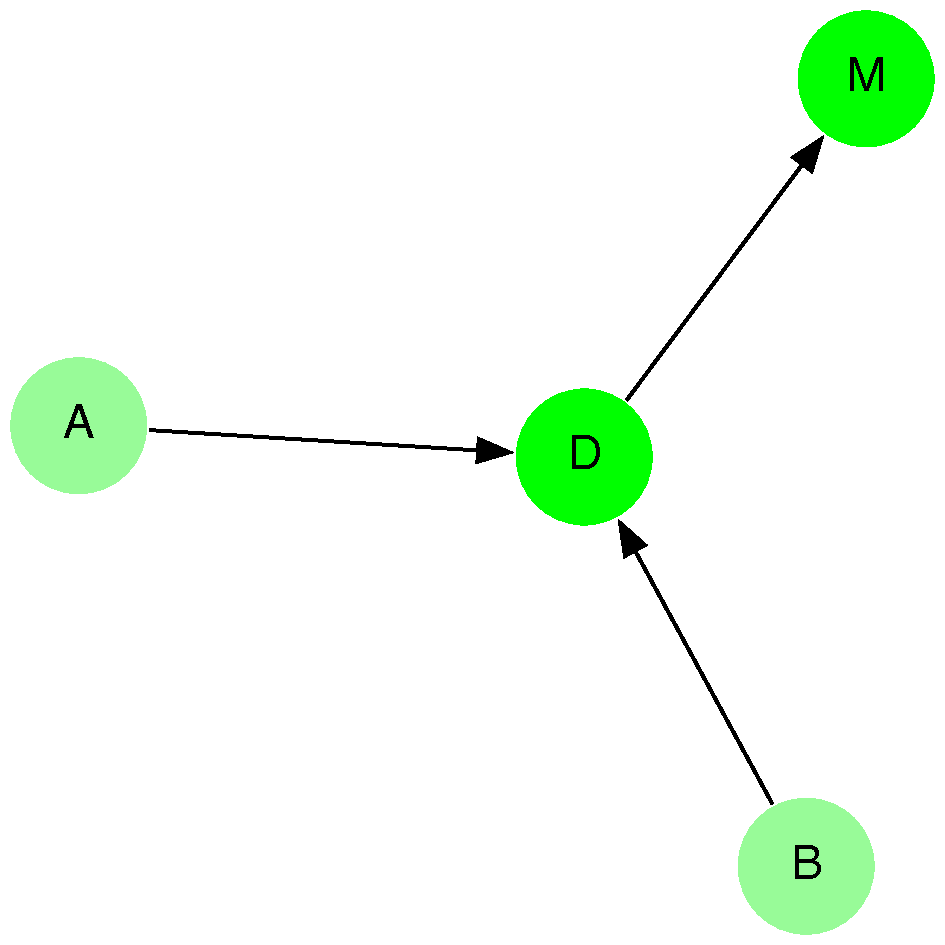
\includegraphics[width=\linewidth]{imgs/pdfs/6_imprecise_rbn.pdf}
        \caption{Associated rBN where model node \textit{M} is imprecise}\label{1_imp_rbn_example}
    \end{subfigure}
    \caption{Example of reduction of eBN with imprecise probabilities}\label{3_imp_reduction}
\end{figure}

\begin{table}[!ht]
    \begin{center}
    \caption{CPTs of the eBN with imprecise probabilities}\label{1_example_CPTs_imprecise}
        \begin{tabular}{P{1.2cm}P{7.8cm}}
            \toprule
            \textbf{Node} & \textbf{CPT} \\
            \midrule
            C & $Pbox\{Normal\}(\mu=[-0.5;0.5];\sigma=[0.8;1.2])$
            \\
            \midrule
            D & 
                \begin{tabular}{P{2.5cm}P{1.5cm}P{1.5cm}}
                    \textbf{scenario} & \:d1 & \:d2 \\
                    \midrule
                    \:a1 \:b1 & $[0.3;0.5]$ & $[0.5;0.7]$ \\
                    \:a1 \:b2 & $[0.0;0.2]$ & $[0.8;1.0]$ \\
                    \:a2 \:b1 & $[0.4;0.6]$ & $[0.4;0.6]$ \\
                    \:a2 \:b2 & $[0.4;0.6]$ & $[0.4;0.6]$ \\
                \end{tabular}
            \\
            \midrule
            M & \begin{tabular}{p{3.3cm}}
                    M:\ $f(d,c) = d - c$ \\
                    P:\ $1-f(d,c) < 0$\\
                \end{tabular}
                \\
        \end{tabular}
    \end{center}
\end{table}

\begin{table}[hbt!]
    \begin{center}
        \caption{CPT of the node \textit{M} after being evaluated in the imprecise eBN}\label{imp_Mnode_tab}
        \begin{tabular}{P{2cm}P{2cm}P{2cm}}
            \textbf{scenarios} & \textbf{$M fail$} & \textbf{$M safe$} \\
            \midrule
            $d1$ & $[0.02;0.6]$ & $[0.4;0.98]$ \\
            $d2$ & $[0.12;0.76]$ & $[0.24;0.88]$ \\
        \end{tabular}
    \end{center}
\end{table}

In the proposed approach, epistemic uncertainties are incorporated into the eBN framework by extending discrete and continuous nodes through imprecise probability theory.
For discrete nodes, the traditionally crisp probability values assigned to each possible state are replaced by probability intervals~\cite{weichselberger_theory_2000}, as for node \textit{D} in Fig.~\ref{1_imp_ebn}. 
This replacement captures the inherent uncertainty in probability estimation, reflecting situations where precise probability values cannot be determined. Similarly, for continuous nodes, traditional univariate PDFs are generalized into either probability boxes~\cite{ferson_2003} or probability intervals that refer to the quantity of interest itself, rather than a probability value as seen for discrete nodes. 
For example, node \textit{C} in Fig.~\ref{1_imp_ebn} illustrates this approach, enabling a more flexible representation of uncertainty in continuous distributions.\\

The presence of imprecise nodes, i.e.\ nodes with imprecise CPTs, introduces two main consequences for the analysis of the network. 
First, whenever a continuous node is imprecise, traditional SRMs, such as First Order Reliability Methods (FORM), Monte Carlo simulations, or Advanced Monte Carlo simulations, are no longer directly applicable for evaluating functional nodes. 
Instead, alternative methods, such as DoubleLoop simulation or Random Slicing~\cite{ALVAREZ_randomslicing}, must be employed to appropriately handle the imprecision in the continuous variables. 
The presence of imprecise parents for functional nodes means that these nodes are defined by a CPT that includes interval values for both failure and safe state probabilities. In the reduction process shown in Fig.~\ref{3_imp_reduction} the nodes CPTs are presented in Tab.~\ref{1_example_CPTs_imprecise} and the resulting failure probability intervals are those in Tab.~\ref{imp_Mnode_tab}. 
This approach allows for a more flexible and accurate analysis of systems where uncertainty is present, particularly when dealing with imprecise inputs and uncertain model parameters.

\begin{figure}[H] 
    \centering
    \begin{minipage}{0.5\textwidth} 
        \centering
        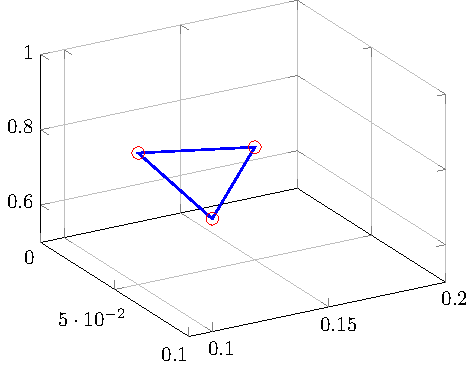
\includegraphics[width=\linewidth]{imgs/pdfs/7_polytope.pdf}
        \caption{Extreme points of the polytope identified by the CPT in Tab.\ref{3_cpt_extremepoints}}\label{3_extreme_points}
    \end{minipage}
    \hfill
    \begin{minipage}{0.4\textwidth}
        \centering
        \begin{tabular}{P{1cm}P{1.5cm}}
            \toprule
            \textbf{states} & \textbf{P} \\
            \midrule
            s1 & $[0.05;0.1]$ \\
            s2 & $[0.1;0.2]$ \\
            s3 & $[0.8;0.9]$ \\
          \end{tabular}
        \captionof{table}{CPT of a discrete imprecise node $S$ with 3 states $s1$, $s2$ and $s3$}\label{3_cpt_extremepoints}
    \end{minipage}
\end{figure}

Whenever a discrete node is imprecise, the rBN is no longer a traditional BN, but instead becomes a Credal Network (CN)~\cite{COZMAN2000199}. 
In the context of CNs, standard exact inference algorithms cannot be directly applied, as the presence of imprecision in the node probabilities introduces a more complex structure. 
To address this, the concept of \textit{strong extension} from the credal set theory~\cite{Levi1980-LEVTEO-7} is employed. 
This extension allows the CN to be decomposed into a set of traditional BNs, each corresponding to one of the extreme points of the n-dimensional polytope in the probability space defined by the intervals of the CPTs of the nodes. This process is illustrated in Fig.~\ref{3_extreme_points}, where each extreme point represents a distinct interpretation of the imprecise probabilities.
Consequently, solving the inference problem for the reduced CN (rCN) of an imprecise eBN requires solving multiple inference problems, one for each extreme point. The result of this process is no longer a single crisp probability value but rather a set of probability bounds, reflecting the uncertainty introduced by the knwoledge imprecision. This is exemplified in Tab.~\ref{imp_inverse_inference_tab}, which shows the probability bounds for nodes \textit{A} and \textit{B} given that node \textit{M} is in a failure state. These bounds provide a more flexible and robust representation of uncertainty, offering a range of possible outcomes instead of a single deterministic probability, thereby capturing the effects of imprecise information in the network.

\begin{table}[hbt!]
    \begin{center}
        \caption{Inverse inference results on nodes \textit{A} and \textit{B} given node \textit{M} in a failure state}\label{imp_inverse_inference_tab}
        \begin{tabular}{P{1.5cm}P{4cm}}
            \textbf{Query} & \textbf{$P(Query | M = M fail)$} \\
            \midrule
            $A = a1$ & $[0.281, 0.673]$ \\
            $A = a2$ & $[0.327, 0.719]$ \\
            $B = b1$ & $[0.205, 0.435]$ \\
            $B = b2$ & $[0.565, 0.795]$ \\
        \end{tabular}
    \end{center}
\end{table}

The examples previously discussed, along with the case study and results presented in the following sections, have been implemented using the Julia library \textit{EnhancedBayesianNetworks.jl}~\cite{ebn.jl}.
    
\section{Case Study}\label{caseofstudy}
    %chktex-file 46
%chktex-file 21
%chktex-file 3
%chktex-file 13
%chktex-file 8
%chktex-file 25

Concrete degradation is a risk factor to account for the long-term performance assessment of radioactive waste disposals, considering their environmental exposure. Over time, degradation processes such as carbonation can lower the alkalinity of concrete, which is essential for protecting the steel reinforcements within these structures from corrosion.
The onset of corrosion can compromise the integrity of containment walls, potentially leading to breaches that could release radioactive contaminants into the environment, and ultimately dose intake.
Properly accounting for these degradation pathways in the performance assessment of radioactive waste repositories over climatic projections is essential for ensuring the containment's longevity and, hence, the protection of public health and the environment. By implementing an eBN, chemical degradation of concrete structures is here evaluated over climatic change projections. 

\subsection{Concrete degradation}
Two most critical degradation processes impacting concrete infrastructure in radioactive waste disposals are carbonation-induced corrosion and chloride-induced corrosion. This section provides a concise overview of both phenomena and presents their respective mathematical models.

\subsubsection{Carbonation-induced corrosion}\label{Carbonation_corrosion_Chpt}
The abundance of $CO_2$ increases the risk of carbonation-induced corrosion in concrete structures~\cite{TALUKDAR_part1,TALUKDAR_part2}. 
The interaction between concrete and atmospheric $CO_2$ causes the formation of calcium carbonate, a process known as carbonation, which reduces the concrete's alkalinity and makes the steel reinforcement in the concrete susceptible to corrosion~\cite{GLASSER2008226}.
Carbonation is quantified by measuring the depth from the concrete surface to where the alkalinity reaches a minimum allowable value. 
Once carbonation reaches the steel reinforcements, the corrosion propagation phase begins, accelerating the degradation of the concrete structure.
In this study, the carbonation depth, denoted as $x_c(t)$, is assessed using the model of~\textcite{Carb_eq_STEWART,Carb_eq_BASTIDASARTEAGA}.
Specifically, Eq.\ref{3:carbonation_depth} describes the increment in carbonation depth $\Delta x_c$ at time $t$, relative to the depth reached at time $t-\Delta T$, where $\Delta T$ denotes the selected evaluation interval in years, e.g., for a decade, $\Delta T = 10$.
\begin{equation}
    \label{3:carbonation_depth}
    \Delta x_c(t, \Delta T) = \sqrt{\frac{2 \ k_{site} \ C_{CO_2}(t) \ f_T^C(t) \ f_{RH}^C(t) \ (D_0^C)^{-n_d}}{a} \ \Delta T} \ \cdot \ \left( \frac{1}{\tau (t, \Delta T)} \right)^{n_m} 
\end{equation}
In defining $\Delta x_c$, $\tau (t, \Delta T)$ is an integer representing the number of $\Delta T$ intervals needed from the reference year to reach the evaluation year $t$, e.g., $t = 2020$ implies $\tau = 1$, $t = 2030$ implies $\tau = 2$, and so on.
The variable $k_{site}$ accounts for potentially higher $CO_2$ concentration values in industrial and urban areas; $C_{CO_2}$ is the time-dependent $CO_2$ concentration measured in \si{\kilogram\per\cubic\meter} is the $CO_2$ diffusion coefficient at reference time $t_0$, measured in \si{\square\meter\per\second}; $n_d$ is the diffusion coefficient aging factor; and $n_m$ is a factor accounting for exposure to microclimatic wetting and drying cycles, with a value of $0$ for sheltered outdoor environments and $0.12$ for unsheltered outdoor. \\
The time-independent quantity $a$ is derived from Eq.\ref{eq_a}, where $\alpha_h$ is the degree of hydration, expressed as a function of the water-to-cement ratio $w / c$. The cement content $Ce$ is measured in \si{\kilogram\per\cubic\meter}, the calcium oxide fraction in cement $CaO$ is approximately 0.65, and the molar masses of $CO_2$ and $CaO$ are \SI{44}{\kilogram\per\mole} and \SI{56}{\kilogram\per\mole}, respectively.
\begin{equation}
    \left\{
    \begin{array}{ll}
    a = 0.75 \ Ce \ CaO \ \alpha_H \frac{M_{CO_2}}{M_{CaO}} \\
      \\
      \alpha_h = 1 - e^{-3.38 \frac{w}{c}}
    \end{array}
    \right.
    \label{eq_a}
\end{equation}
The time-dependent quantities $f_T^C$ and $f_{RH}^C$ allow the incorporation of climate variable effects, associated with climate change projections, into the carbonation depth evaluation, as presented in the analytical models by~\textcite{Carbonation_BASTIDASARTEAGA}. 
Specifically, $f_T^C$ represents the dynamic effect of temperature on carbonation, impacting the diffusion coefficient according to the Arrhenius Law~\cite{Carbonation_YOON}, as shown in Eq.\ref{3:ft}. Here, $E$ is the activation energy of the diffusion process, i.e.,
\SI{38.3}{\kilo\joule\per\mole}; $R$ is the gas constant, i.e., \SI{8.314}{\kilo\joule\per\mole\per\kelvin}; $T(t_0)$ is the reference temperature, i.e.,\SI{293}{\kelvin}; and $T(t)$ is the temperature in Kelvin at time $t$.
\begin{equation}
    \label{3:ft}
        f_T^C (t) = e^{\frac{E}{R} \left[ \frac{1}{T_0} - \frac{1}{T(t)} \right]}
\end{equation}
The effect of relative humidity (RH) has been extensively studied. Research by~\textcite{f_rh_Al-Khaiat} suggests that RH levels below 30\% do not significantly impact carbonation depth, whereas~\textcite{f_rh_BARY} indicates that RH levels above 50\% have a significant influence. For this study, the analytical model chosen to describe the RH effect over time on the diffusion coefficient is the one proposed by~\textcite{Carbonation_BASTIDASARTEAGA}, detailed in Eq.\ref{3:frh}.
\begin{equation}
    \left\{
    \begin{array}{ll}
    0 & if \ RH \leq 0.25\\
    \left[\frac{1-RH(t)^\beta}{1-RH_0^\beta} \right]^\alpha & otherwise
    \end{array}
    \right.
    \label{3:frh}
\end{equation}
Here, $RH_0$ is the reference value for RH, whereas $\alpha$ and $\beta$ are independent parameters of exposure conditions. In this case study, the reference RH is set to 0.65, $\alpha$ is 5 and $\beta$ is 2.5.

\subsubsection{Chloride-induced corrosion}\label{Chloride_corrosion_Chpt}
The penetration and movement of chloride ions into concrete structures involve the electrochemical dissolution of iron, leading to the degradation of concrete barriers.
Chloride ingress into concrete is typically described using a diffusion model, which is a single mass transport equation for chloride ion transport.
In this study, a time-dependent model is applied, incorporating the chloride diffusion coefficient to estimate chloride concentration over time. The chloride concentration at a depth $z$ and time $t$ is described by Eq.~\ref{eq:chloride_corrosion}.
\begin{equation}
    \label{eq:chloride_corrosion}
    C(z, t) = C_0^{Cl} \left[ 1-erf \left(\frac{z}{2\sqrt{k_e \ k_t \ k_c \ f_T^{Cl}(t) \ f_{RH}^{Cl}(t) \ D_0^{Cl} \ \omega \ \tau(t, \Delta T)}} \right) \right]
\end{equation}
Here, $C_0^{Cl}$ represents the chloride concentration at the boundary; for atmospheric areas remote from coasts, $C_0^{Cl}$ is typically around \SI{1.15}{\kilogram\per\cubic\meter}, whereas, in coastal or tidal areas, the chloride concentration at the surface is significantly higher. $D_0^{Cl}$ is the reference chloride diffusion coefficient; $k_e$ is the environmental coefficient; $k_t$ is the test method factor and $k_c$ is the curing factor. 
Coefficient $\omega$ represents the number of seconds in 10 years whereas $\tau(t, \Delta T)$ has the same definition given in Sec.~\ref{Carbonation_corrosion_Chpt}.\\
Similar to carbonation, there are two time-dependent quantities that account for the effects of climate change projections on temperature and relative humidity: $f_{T}^{Cl}$ and $f_{RH}^{Cl}$.
\begin{equation}
    \label{eq_f_rh_cl}
    f_{RH}^{Cl}(t) = \left[ 1 + \frac{(1-RH(t))^4}{(1-RH_0)^4} \right]^{-1}
\end{equation}
The temperature effect is consistent with that defined for carbonation in Eq.\ref{3:ft}, thus $f_T^C = f_T^{Cl}$. The effect of RH is expressed in the work of~\textcite{f_RH_ClELHASSAN} as shown in Eq.\ref{eq_f_rh_cl}.

\subsection{eBN for concrete degradation}
The eBN framework is exemplified to perform the analysis of concrete degradation over climatic change projections. 
Climate change data are taken from the catalogue provided in~\textcite{Copernicus_Climate_Change} and include three main projection scenarios referred to three different Shared Socio-economic Pathways, namely \textit{ssp1}, \textit{ssp2} and \textit{ssp5}. 
These projections account for variations in temperature, $CO_2$ concentration and relative humidity from 2020 to 2100, relevant for concrete corrosion models.\\ 
In this study, the eBN integrates the two degradation models presented in~\ref{Carbonation_corrosion_Chpt} and in~\ref{Chloride_corrosion_Chpt}, and is structured to capture the probabilistic dependencies considering epistemic and aleatoric uncertainties, between climate conditions of temperature, relative humidity and $CO_2$ concentration, material properties, e.g.~diffusion coefficients, water-to-cement ratio and the final state of the system, through the carbonation and chloride effects on concrete.
The following sections detail the eBN structure, the probabilistic modelling of input variables and its application to the case study of a radioactive waste disposal concrete structures degradation. 
Initially, the carbonation-induced and chloride-induced corrosion models are examined separately to enhance clarity and comprehensibility. 
Subsequently, the complete eBN framework, integrating both degradation mechanisms, is presented.

\subsubsection{eBN -- Carbonation-induced corrosion model}\label{ebn_carbonation_section}
The eBN representing the carbonation process, illustrated in Fig.~\ref{carbonation_ebn}, includes two primary discrete root nodes. The first is the node \textit{t}, which denotes the selected time slice (considering $\Delta T$ equals to a decade); it consists of nine equally probable states, corresponding to the decades from 2020 to 2100. The second node, \textit{proj}, represents the climate change projections, with three equally likely states, each associated with an \textit{ssp} (i.e~\textit{ssp1}, \textit{ssp2} and \textit{ssp5}).
\begin{figure}[H]
    \centering
    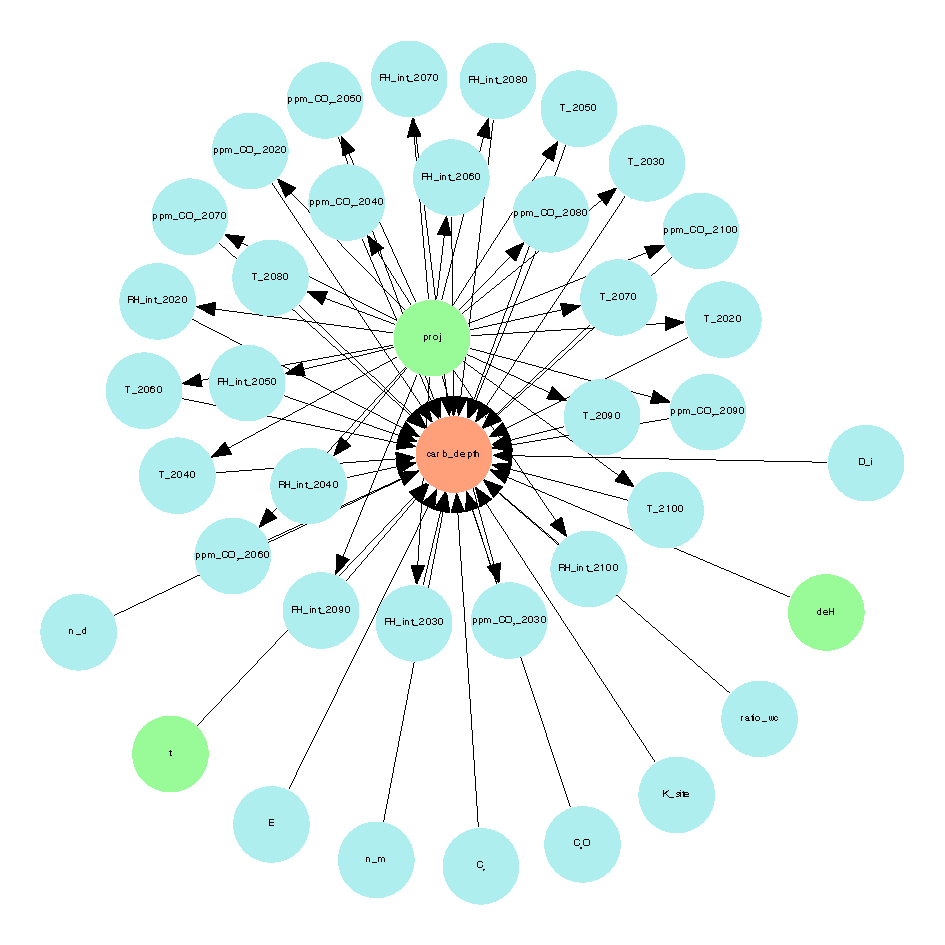
\includegraphics[width=\linewidth]{imgs/pdfs/8_carb_ebn.pdf}
    \caption{Carbonation-induced corrosion eBN with precise nodes}\label{carbonation_ebn}
\end{figure}
A third discrete root node, \textit{DeH}, is also shown in Fig.~\ref{carbonation_ebn}. This node represents a control variable to reduce the RH below a threshold. Specifically, whenever RH exceeds 0.25, the node enforces a reduction to 0.2. These values were selected based on the influence of RH on the carbonation model, as illustrated in Fig.~\ref{carbonation_depth vs RH}.
\begin{figure}[H]
    \centering
    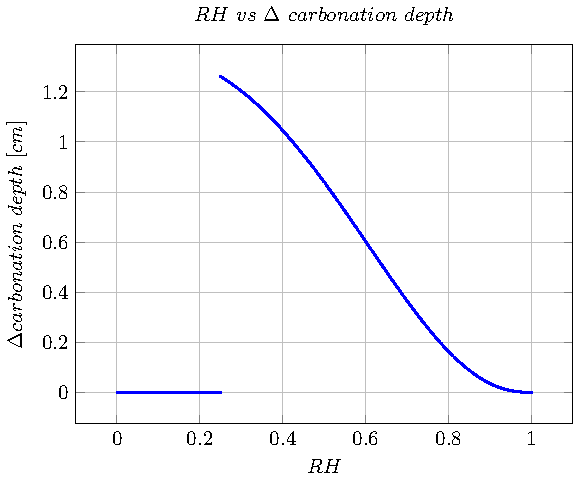
\includegraphics[scale=0.7]{imgs/pdfs/10_RH_carb.pdf}
    \caption{RH effect on carbonation depth}\label{carbonation_depth vs RH}
\end{figure}
The \textit{DeH} node is modelled as a Boolean variable with two states: failed ($P_{F} = 10^{-4}$) and working ($P_{W} = 1 - 10^{-4}$). \\
In addition, eight continuous root nodes are introduced to account for aleatoric uncertainties in the parameters $n_d$, $n_m$, $E$, $k_{site}$, water-to-cement ratio ($w/c$), $C_e$, $CaO$ and $D_0^C$. Their CPTs are provided in Table~\ref{continuous_root_node_ebn_carb}.
\begin{table}[hbt!]
    \begin{center}
        \caption{Distribution of the continuous root nodes of the eBN depicted in Fig.\ref{carbonation_ebn}}\label{continuous_root_node_ebn_carb}
        \begin{tabular}{P{2cm}P{2.2cm}P{6cm}}
            \textbf{Quantity} & \textbf{Node Name} & \textbf{Distribution} \\
            \midrule
            $n_d$       & $n \_ d$          & $Trunc(N(0.24;2.88e^{-2}); 0, \infty)$ \\
            $n_m$       & $n \_ m$          & $Trunc(N(0.12;1.2e^{-2}); 0, \infty)$\\
            $E$         & $E$               & $Uniform(34.853;41.747)$ \\
            $k_{site}$  & $k \_ site$       & $Trunc(N(1.15;1.15e^{-2}); 0, \infty)$ \\
            $w / c$     & $ratio \_ w/c$    & $Trunc(LogN(-0.69; 0.05); 0, 1)$ \\
            $Ce$        & $C_e$             & $Trunc(N(300;30); 0, \infty)$ \\
            $CaO$       & $C_aO$            & $Uniform(0.585; 0.715)$ \\
            $D_0^C$     & $D \_ i$          & $Trunc(N(2.2e^{-4};1.5e^{-5}); 0, \infty)$ \\
        \end{tabular}
    \end{center}
\end{table}
The carbonation process is governed by the model presented in Eq.~\ref{3:carbonation_depth}, which explicitly depends on temperature, $CO_2$ concentration and RH. 
These variables are characterized through climate change projections data for a nuclear waste disposal located in Belgium (see Appendix~\ref{appendixA}). \\
The model is dynamic in nature, as its output corresponds to the increment in carbonation depth accumulated over the decade ending in the year under consideration. Therefore, to evaluate the total carbonation depth, one must consider the cumulative sum of increments from all preceding decades.
We have introduced decade-specific nodes for temperature, $CO_2$ concentration (in ppm) and relative humidity over decades.
Examples include $T\_ {2020}$, $T\_ {2030}$ and so on up to $T\_ {2100}$, as shown in Fig.~\ref{carbonation_ebn}. These nodes are all modelled as children of the \textit{proj} node, with distributions detailed in Tables~\ref{Climate_Change_Tnode_dists},~\ref{Climate_Change_RHnode_dists} and~\ref{Climate_Change_CO2node_dists}.
This structure supports the definition of the functional node \textit{carb\_depth}, which is a child of all temperature, $CO_2$ and RH nodes, as well as of \textit{proj}, \textit{DeH} and the time slice node \textit{t}. 
For each time slice, a dedicated model computes the incremental carbonation depth by summing contributions from previous decades. 
If the resulting total exceeds the threshold of 3 cm, defined by~\textcite{Carbonation_BASTIDASARTEAGA}, the system transitions to a failure state. 
In the carbonation model, the inputs from the $ratio\_w/c$ node and all the RH percentage change nodes are modified before being passed to the computational component. 
Specifically, the $ratio\_w/c$ samples are scaled by a factor of 0.1 and then shifted by +0.5, whereas the RH percentage change samples are randomly assigned as either positive or negative deviations from the reference RH.

\subsubsection{eBN -- Chloride-induced corrosion model}\label{ebn_chloride_section}
The chloride-induced corrosion process is represented by the eBN depicted in Fig.~\ref{chloride_ebn}. This model includes some of the same continuous nodes as the corrosion process eBN, specifically for temperature, $CO_2$ concentration, RH. It also shares the  discrete nodes \textit{proj}, \textit{t} and \textit{DeH}. The effect of relative humidity on the chloride penetration is shown in Fig.~\ref{RH vs chloride depth}.
\begin{figure}[H]
    \centering
    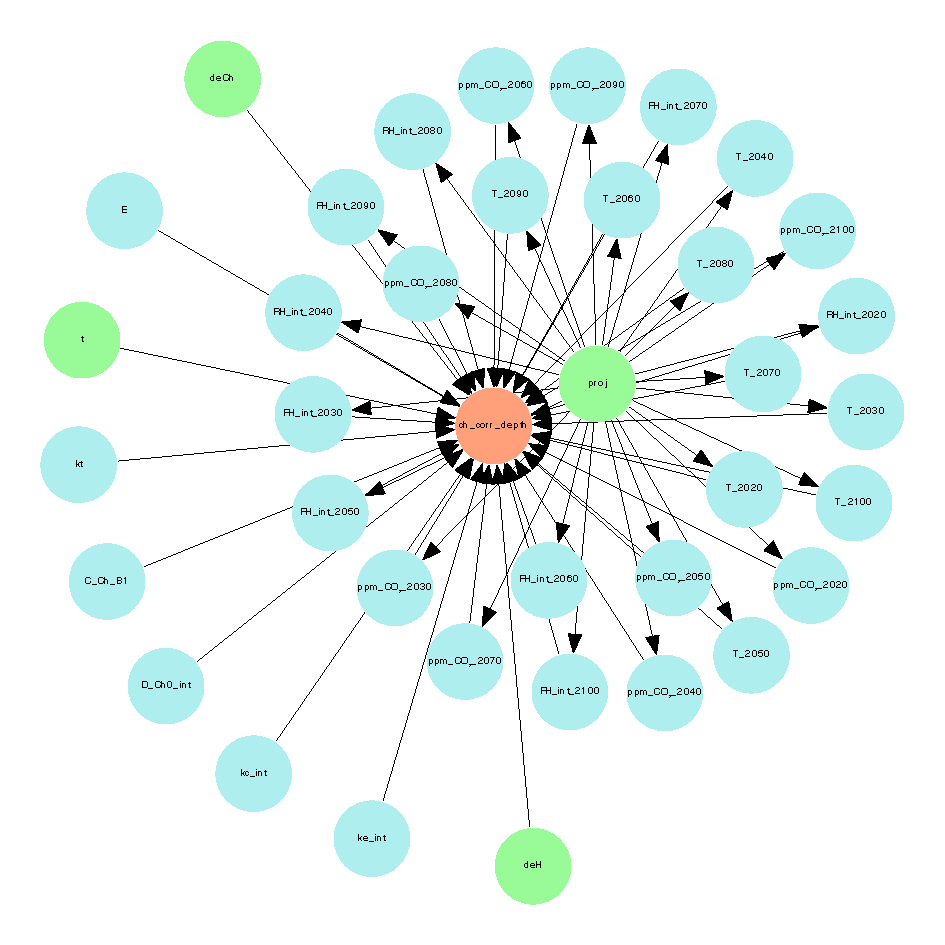
\includegraphics[width=\linewidth]{imgs/pdfs/9_chloride_ebn.pdf}
    \caption{Chloride-induced corrosion eBN with precise nodes}\label{chloride_ebn}
\end{figure}
\begin{figure}[H]
    \centering
    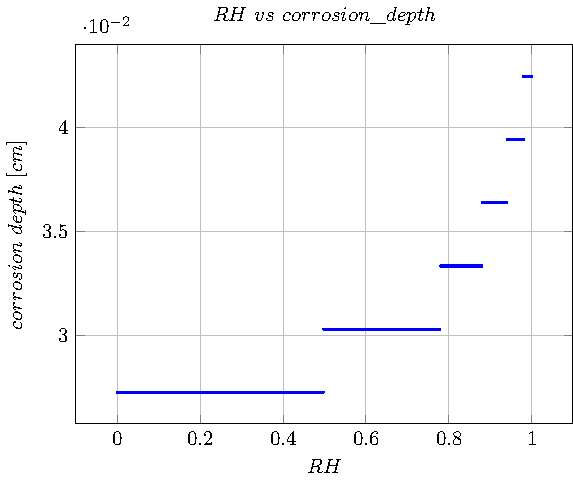
\includegraphics[scale=0.7]{imgs/pdfs/11_RH_corr.pdf}
    \caption{RH effect on chloride penetration depth}\label{RH vs chloride depth}
\end{figure}
\begin{figure}[H]
    \centering
    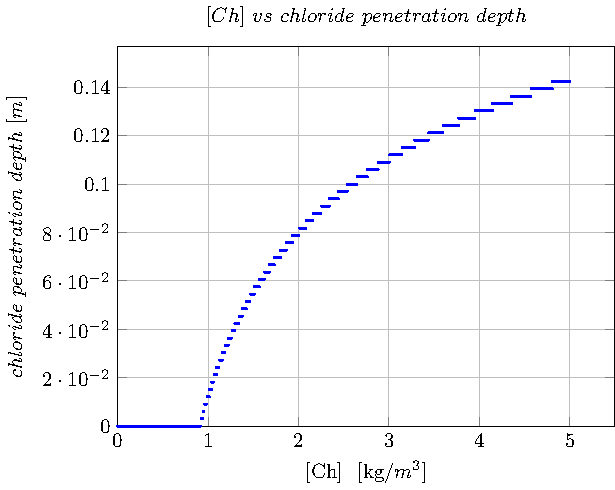
\includegraphics[scale=0.7]{imgs/pdfs/11_Chloride_corr.pdf}
    \caption{Chloride concentration at system boundary effect on chloride penetration depth}\label{Chloride vs corrosion depth}
\end{figure}

\textit{DeCh} is a discrete root node that represents a chloride mitigation control variable that reduces the boundary chloride concentration, $C_0^{Cl}$, when it exceeds a critical level.
The effect of the boundary chloride concentration on the model is shown in Fig.~\ref{Chloride vs corrosion depth}. $DeCh$ node is modelled as a Boolean variable with states \textit{working} and \textit{failed}, with assigned probabilities $P_W = 1 - 10^{-4}$ and $P_F = 10^{-4}$, respectively. It is designed to lower $C_0^{Cl}$ from values above 0.9 to 0.7. \\
Five continuous root nodes are also included to represent aleatoric uncertainties in the parameters $k_t$, $k_c$, $k_e$, $C_0^{Cl}$, and the reference diffusion coefficient $D_0^{Cl}$. Their distributions are detailed in Table~\ref{continuous_root_node_ebn_ch}.

\begin{table}[hbt!]
    \begin{center}
        \caption{Continuous root node distribution of the eBN in Fig.\ref{chloride_ebn}}\label{continuous_root_node_ebn_ch}
        \begin{tabular}{P{1.6cm}P{2.1cm}P{6cm}}
            \textbf{Quantity} & \textbf{Node Name} & \textbf{Distribution} \\
            \midrule
            $k_t$       & $kt \_ int$      & $Trunc(N(0.832;2.4e^{-2}); 0, \infty)$ \\
            $k_e$       & $ke \_ int$      & $Gamma(2;1)$ \\
            $k_c$       & $kc \_ int$      & $Beta(2;2)$ \\
            $C_0^{Cl}$  & $C\_ Ch\_ B1$    & $Trunc(N(1.15; 0.675); 0, \infty)$~\cite{Carb_eq_STEWART}\\
            $D_0^{Cl}$  & $D\_ Ch0\_ int$  & $Trunc(LogN(0;0.5); 0, 1)$ \\
        \end{tabular}
    \end{center}
\end{table}

As with the \textit{ratio\_w/c} node and RH percentage change nodes in~\ref{ebn_carbonation_section}, the outputs of \textit{ke\_int}, \textit{kc\_int}, and \textit{D\_Ch0\_int} are transformed before use in the computational model. Specifically:
- \textit{ke\_int} samples are scaled by 0.155 and shifted by +0.924;
- \textit{kc\_int} samples are scaled by 0.7 and shifted by +2.4;
- \textit{D\_Ch0\_int} samples are scaled by 0.2, shifted by +1, and multiplied by $6 \times 10^{-12}$.

All these nodes feed into the \textit{ch\_corr\_depth} node, which uses the model in Eq.~\ref{eq:chloride_corrosion} to evaluate the chloride concentration $C(z;t)$ across the concrete depth. 
Unlike the carbonation model, this model is not time-recursive but spatially dependent in the z-direction. The chloride penetration depth is defined as the depth at which $C(z;t)$ first reaches \SI{0.9}{\kilogram\per\cubic\meter}~\cite{fuma}.
This depth is compared against a failure threshold of \SI{12}{\centi\meter} to assess structural safety.
Further implementation details of the \textit{ch\_corr\_depth} node can be found in the associated code repository.

\subsubsection{eBN -- Concrete corrosion}
The final eBN embeds two corrosion models as depicted in Fig.~\ref{fig:precise_ebn}. Nodes associated to temperature, $CO_2$ concentration and RH are shared, as well as the \textit{proj}, \textit{DeH} and \textit{t} nodes. 

\begin{figure}[]
    \centering
    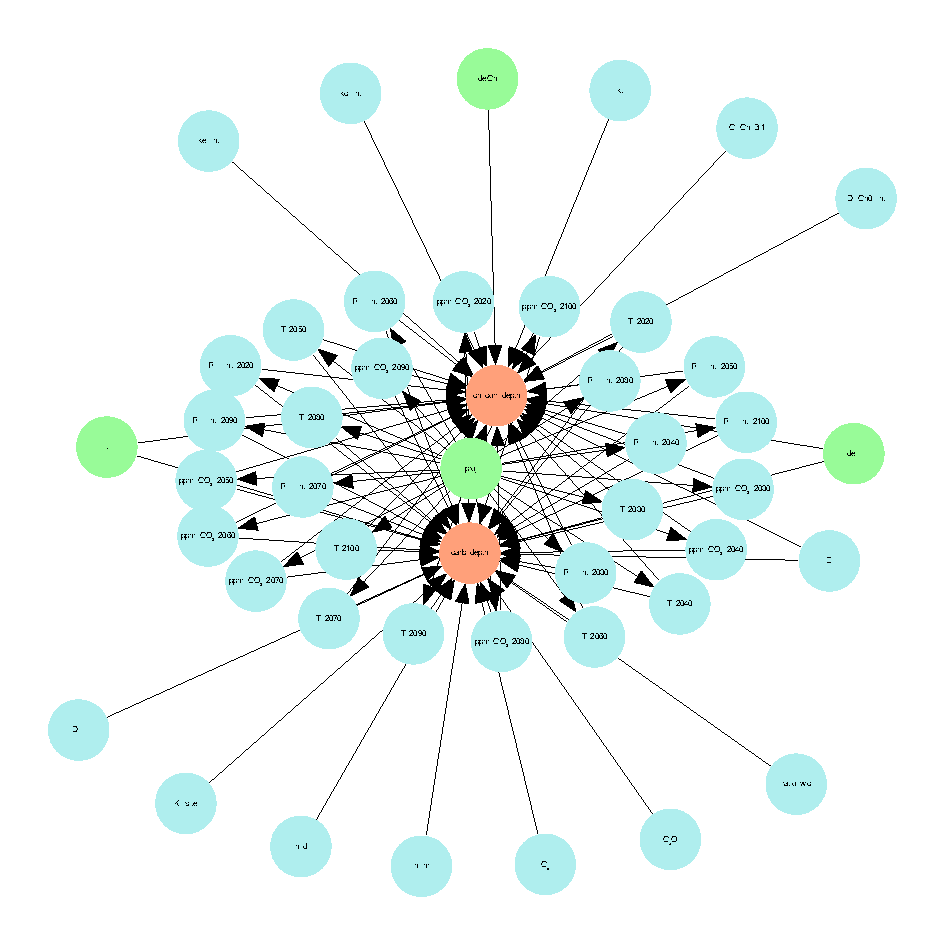
\includegraphics[width=\linewidth]{imgs/pdfs/12_total_ebn_precise.pdf}
    \caption{Concrete corrosion eBN with precise nodes}\label{fig:precise_ebn}
\end{figure}

The functional nodes \textit{ch\_corr\_depth} and \textit{carb\_depth} are initially defined through the set of continuous random variables coming from their continuous parents, the set of discrete random variables coming from their discrete parents and a simulation technique, selected to be a standard Monte Carlo with $10^4$ samples for both of them.
The union of these two sets of inputs together with the chosen simulation technique and two performance functions, allows solving the structural reliability problem. 
In this way, it is possible to obtain the two CPTs associated with the two discrete nodes \textit{ch\_corr\_depth} and \textit{carb\_depth} in the reduced BN of Fig.~\ref{fig:precise_rbn}. 

\begin{figure}[H]
    \centering
    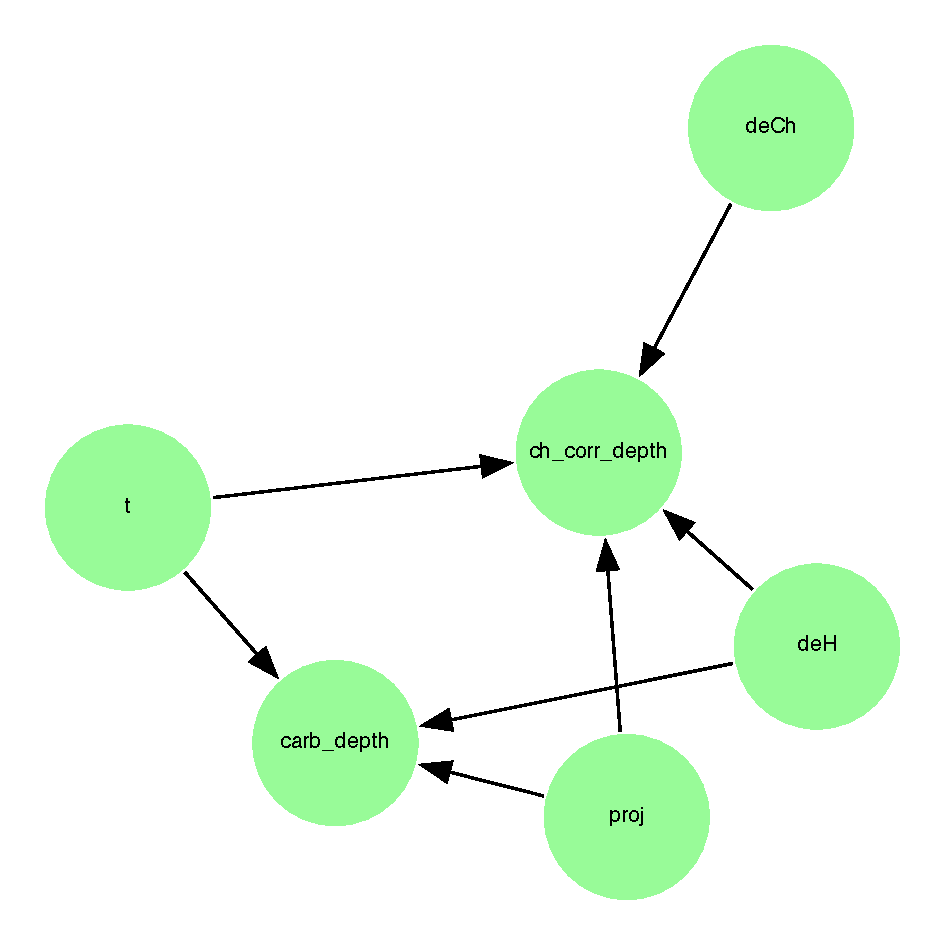
\includegraphics[scale=0.5]{imgs/pdfs/13_total_rbn_precise.pdf}
    \caption{Concrete corrosion risk rBN with precise nodes}\label{fig:precise_rbn}
\end{figure}

In this BN, only discrete nodes are present. Both \textit{ch\_corr\_depth} and \textit{carb\_depth} have as parents the discrete nodes referred to the specific time slice, to the specific climatic projection and the auxiliary discrete node \textit{deH}. The node \textit{deCh} influences the sole node chloride-induced corrosion process, therefore it is not a parent of \textit{carb\_depth}.

\subsubsection{Imprecise eBN -- Imprecision in climatic change data}

In the climatic change data catalogue~\cite{Copernicus_Climate_Change}, each \textit{ssp} comes from different down-scaled regional climatic models (RCMs). The Gaussian distributions defined in Tab.~\ref{Climate_Change_Tnode_dists},~\ref{Climate_Change_RHnode_dists} and~\ref{Climate_Change_CO2node_dists} have been extrapolated based on limited number of RCMs.
A more robust way for dealing with the epistemic uncertainty problem of future projections is represented by the interval probability theory. Therefore, without introducing any hypothesis over the specific distribution, the quantities of interest have been treated as interval values, i.e.~defined only by an upper bound and a lower bound, given respectively by the maximum and minimum values of all the simulations related to a specific \textit{ssp}.

\begin{figure}[H]
    \centering
    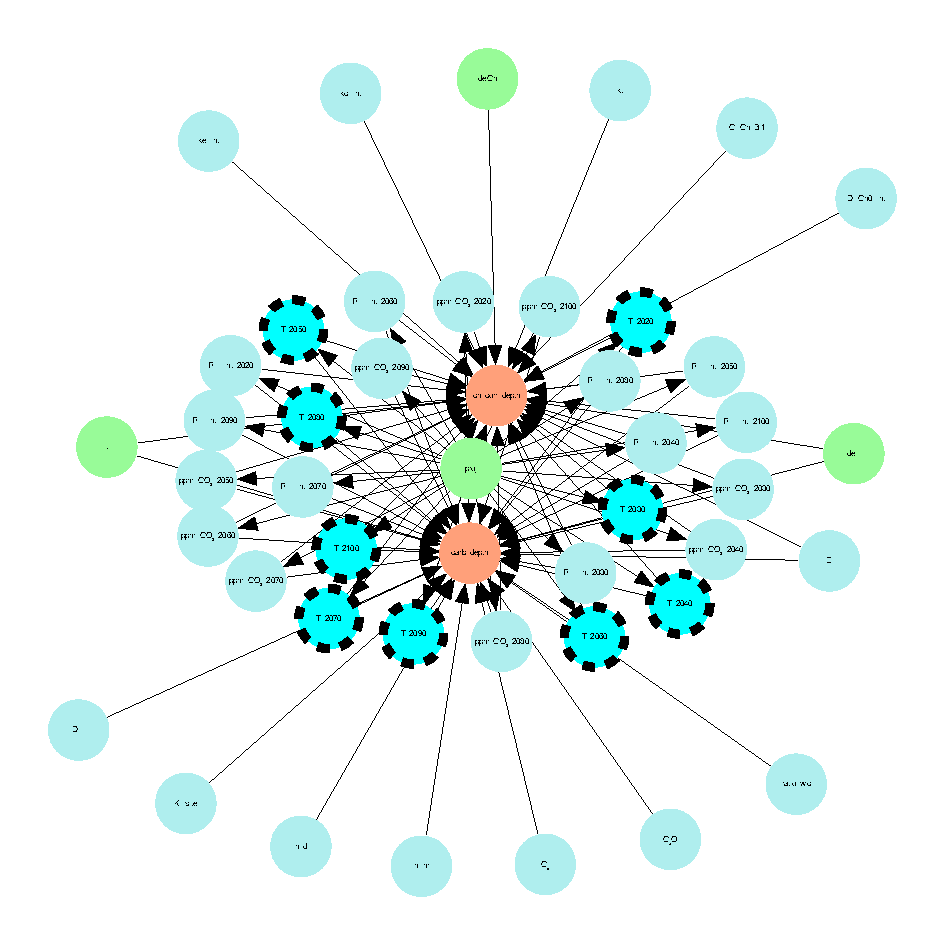
\includegraphics[width=\linewidth]{imgs/pdfs/14_total_ebn_imprecise.pdf}
    \caption{Concrete corrosion eBN with imprecise temperature nodes}\label{fig:imprecise_ebn}
\end{figure}

This concept has been applied to the temperature projections obtaining the new node presented in Fig.~\ref{fig:imprecise_ebn} and defined in Tab.~\ref{Climate_Change_Tnode_interval}. The reduced BN of this imprecise eBN is the Credal Network presented in Fig.~\ref{fig:imprecise_rbn}.
\begin{figure}[H]
    \centering
    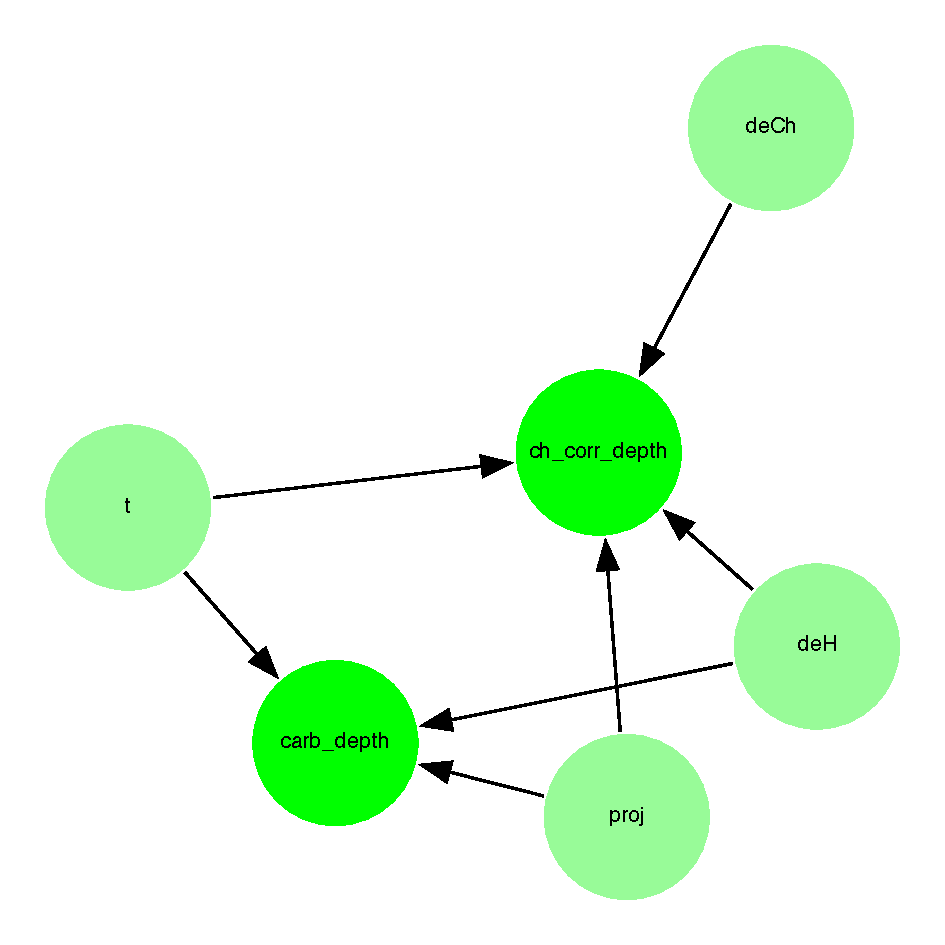
\includegraphics[scale=0.5]{imgs/pdfs/15_total_rbn_imprecise.pdf}
    \caption{Concrete corrosion risk rBN with imprecise nodes}\label{fig:imprecise_rbn}
\end{figure}

\section{Results \& Discussions}\label{results}
    %chktex-file 46
%chktex-file 21
%chktex-file 3
%chktex-file 13
%chktex-file 8
%chktex-file 25

This section presents a comprehensive discussion of the results obtained from the application of the eBN framework addressing the relevant uncertainties in the concrete corrosion, with a particular focus on imprecise data arising from climate change projections. Before delving into these findings, we first summarize the outcomes of the sensitivity analysis (SA) performed on the carbonation-induced and chloride-induced corrosion processes.

\subsection{Sensitivity Analysis of concrete corrosion processes}
SA has been perfomed to identify the most influential factors affecting concrete corrosion processes.
% SA is vital for the efficiency of a probabilistic risk assessment tool, as it enables the exclusion of variables with minimal impact on outcomes, thereby reducing the computational demands of the risk assessment framework.
Sobol' indices are used and reliable indices for global SA.0 
This choice is justified because of their rigorous theoretical foundation in variance-based decomposition, the ability to capture both linear and nonlinear dependencies, including high-order interactions among random variables and the clear interpretability~\cite{Sobols_indices_SOBOL}.
Sobol' indices have been evaluated for both corrosion models to rank the effect of the random variables on the outputs. 

\subsubsection{Carbonation-induced corrosion}\label{SA_carbonation}
The random variables considered in the SA of the carbonation model are the same as those introduced in Sec.~\ref{ebn_chloride_section}. 
The variables \textit{Ce}, \textit{Ca}, \textit{k\_site}, \textit{n\_d}, \textit{n\_m}, \textit{E}, \textit{ratio\_wc} and \textit{D\_i} follow the same probability distribution across all decades and climatic projections, whereas the distributions of \textit{T}, \textit{ppm\_CO\textsubscript{2}} and \textit{RH\_int} vary depending on the decade and climate projection. \\ 
Figure~\ref{Sobol_carb_2020ssp1} shows the Sobol' indices for the carbonation model during the first decade under the \textit{ssp1} climate scenario. 
Both the first-order and total-effect Sobol' indices are negligible for all input variables except for relative humidity, indicating that \textit{RH\_int} is the only variable that significantly contributes to the output variance, both independently (first-order effect) and through interactions with other variables (total effect).
Sobol' indices have been computed for each decade and for all considered climate projections. The results consistently exhibit the same trend as illustrated for the first-decade and \textit{ssp1} projection, with relative humidity remaining the dominant factor influencing output variance. 

\begin{figure}[H]
    \centering
    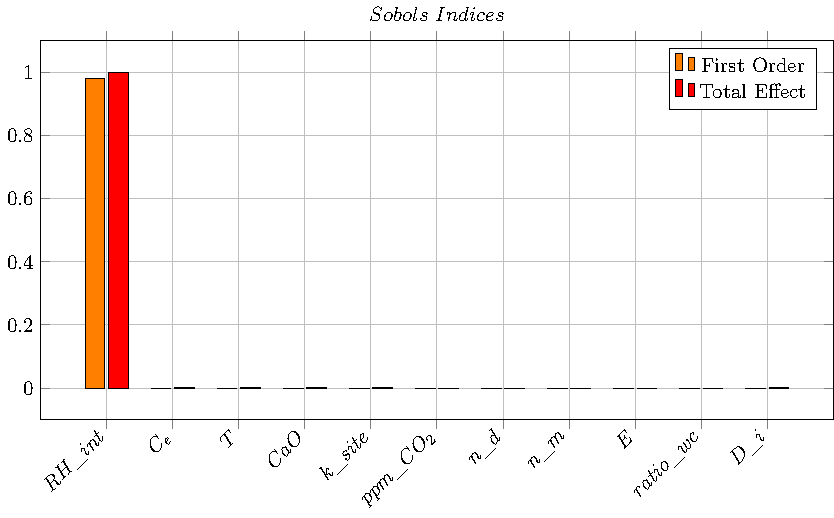
\includegraphics[width=0.8\linewidth]{imgs/pdfs/sobols_indices/carbonation/17_sobols_2020_ssp1.pdf}
    \caption{Sobol' indices of the model for carbonation-induced corrosion considering the random variables identified by the year 2020 and the projection \textit{ssp1}}\label{Sobol_carb_2020ssp1}
\end{figure}
In Fig.~\ref{Sobol_carb_2020uniform}, Sobol' indices are presented under the assumption that all input variables follow uniform probability distributions. For the variables \textit{Ce}, \textit{Ca}, \textit{k\_site}, \textit{n\_d}, \textit{n\_m}, \textit{E}, \textit{ratio\_wc}, and \textit{D\_i}, the uniform distribution bounds were defined as the minimum and maximum values obtained from $10^4$ samples drawn from their respective original distributions. For the time-dependent variables \textit{T}, \textit{ppm\_CO\textsubscript{2}}, and \textit{RH\_int}, the uniform bounds for each decade were derived from the minimum and maximum of a merged set of $3 \times 10^4$ samples, aggregated across all climate change projections. This approach is adopted to enhance the potential influence of the distribution tails, particularly those of the original Gaussian distributions, thereby allowing a more comprehensive assessment of the input variables' impact on model output variability. 
The analysis confirms that relative humidity continues to exert the most significant influence on the variability of the model output, even under the assumption of uniformly distributed inputs.
\begin{figure}[H]
    \centering
    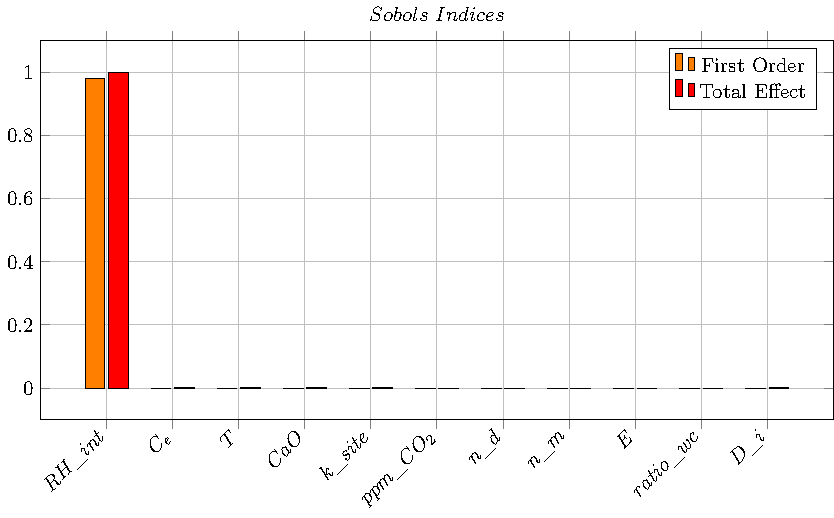
\includegraphics[width=0.8\linewidth]{imgs/pdfs/sobols_indices/carbonation/17_sobols_2020_ssp1.pdf}
    \caption{Sobol' indices of the model for carbonation-induced corrosion at year 2020 under the uniform distributions assumption}\label{Sobol_carb_2020uniform}
\end{figure}

\subsubsection{Carbonation-induced corrosion}
The same procedure presented in Sec.~\ref{SA_carbonation} has been applied to the chloride-induced corrosion model, obtaining the results presented in Fig.~\ref{Sobol_ch_2020ssp1} and Fig.~\ref{Sobol_ch_2020uniform}.
\begin{figure}[H]
    \centering
    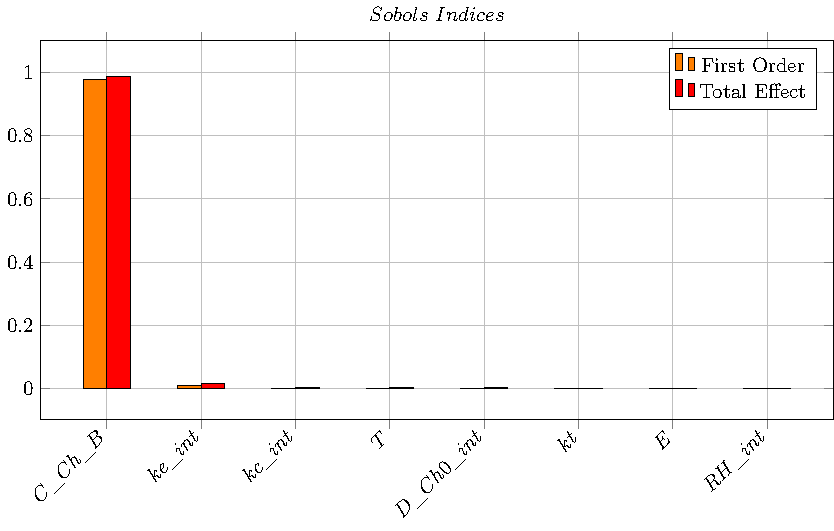
\includegraphics[width=0.8\linewidth]{imgs/pdfs/sobols_indices/chloride/19_sobols_withRH_2020_ssp1.pdf}
    \caption{Sobol' indices of the model for chloride-induced corrosion considering the random variables identified by the year 2020 and the projection \textit{ssp1}}\label{Sobol_ch_2020ssp1}
\end{figure}

\begin{figure}[H]
    \centering
    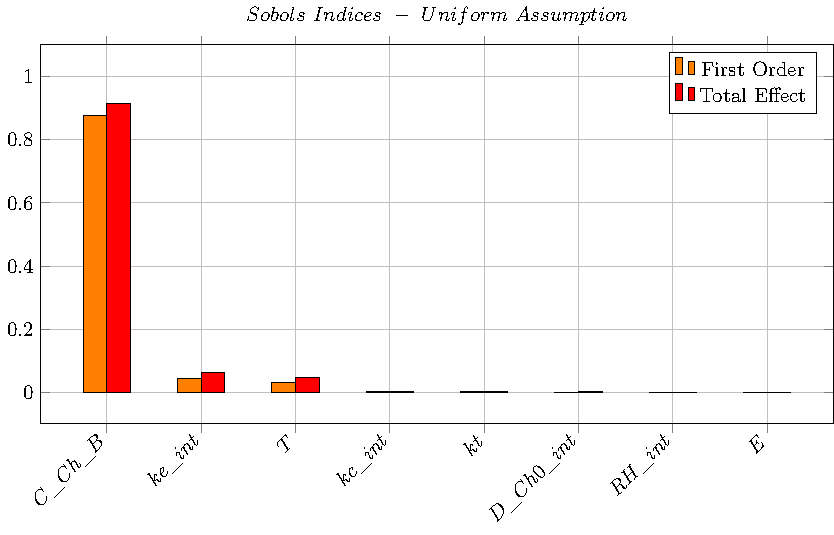
\includegraphics[width=0.8\linewidth]{imgs/pdfs/sobols_indices/chloride/18_sobols_withRH_uniform_2020.pdf}
    \caption{Sobol' indices of the model for chloride-induced corrosion at year 2020 under the uniform distributions assumption}\label{Sobol_ch_2020uniform}
\end{figure}
For the chloride-induced corrosion model, relative humidity is identified as the primary driver of output variability in both distributional scenarios. However, under the uniform input assumption, additional factors such as temperature, the curing factor and the environmental factor also exhibit a non-negligible influence on the output variance.

\subsection{Exceedance Probabilities for Corrosion}

The results of the SA motivated the introduction of two control nodes, \textit{DeH} and \textit{DeCh}, to regulate relative humidity and chloride concentration at the system boundaries. 
These nodes are defined as follows.
The node \textit{DeH} represents a dehumidifier unit, modelled as a root node with a failure probability of $10^{-4}$ and is parent to both the model nodes.
Its influence is identical across the two models: when operational (i.e., not in a failed state) and when the relative humidity exceeds a specified threshold, it reduces the humidity to a defined target level. 
In the eBN described in Sec.~\ref{caseofstudy}, the threshold and target relative humidity values are set to 0.25 and 0.2, respectively.
The node \textit{DeCh} is conceptually similar to \textit{DeH}.
It is also a root node with a failure probability of $10^{-4}$ and is defined by a threshold and target value for chloride concentration. 
Unlike \textit{DeH}, \textit{DeCh} influences only the chloride-induced corrosion model, where it acts to reduce the chloride concentration at the system boundary when the threshold is exceeded. 
In the eBN presented in Sec.~\ref{caseofstudy}, the threshold and target chloride concentration values are 0.9 and 0.7, respectively.\\

\subsubsection{Precise eBN}
Exceedance probabilities for corrosion are contained in the CPTs of the two functional of the eBNs presented in Sec.\ref{caseofstudy}. 
Results for the precise eBN depicted in Fig.~\ref{fig:precise_ebn} are obtained through Monte Carlo simulation with $10^4$ samples and considering a maximum allowed carbonation depth of \SI{3}{\centi\meter} and a maximum allowed chloride penetration of \SI{12}{\centi\meter}, where the chloride penetration is defined as depth when chloride concentration is larger than \SI{0.9}{\kilogram\per\cubic\meter}, for defining the performance functions of nodes \textit{carb_depth} and \textit{ch_corr_depth}.
In particular the CPT of the carbonation node in the precise rBN depicted in Fig.\ref{fig:precise_rbn} has 54 possible scenarios, identified by 9 decades, 3 projections and 2 possible states of the dehumidifier unit. This CPT shows that whenever the dehumidifier unit is working the carbonation process never reaches the failure threshold, for all the decades before year 2060 the failure never occurs, and after year 2060 failure of the system can take place with the probabilities shown in Tab.~\ref{Carbonation_precise_cpt}.

\begin{table}[H]
    \begin{center}
    \caption{Carbonation-induced corrosion node partial CPT for the precise eBN of Fig.~\ref{carbonation_ebn}}\label{Carbonation_precise_cpt}
        \begin{tabular}{P{6cm}P{4cm}}
            \toprule
            \textbf{scenarios} & \textbf{states probabilities} \\
            \midrule
                \begin{tabular}{P{1.5cm}P{1.5cm}P{1.5cm}}
                    \textbf{t} & \textbf{DeH} & \textbf{proj} \\
                    \midrule
                    2060 & broken & ssp1 \\
                    2060 & broken & ssp2 \\
                    2060 & broken & ssp5 \\
                    2070 & broken & ssp1 \\
                    2070 & broken & ssp2 \\
                    2070 & broken & ssp5 \\
                    2080 & broken & ssp1 \\
                    2080 & broken & ssp2 \\
                    2080 & broken & ssp5 \\
                    2090 & broken & ssp1 \\
                    2090 & broken & ssp2 \\
                    2090 & broken & ssp5 \\
                    2100 & broken & ssp1 \\
                    2100 & broken & ssp2 \\
                    2100 & broken & ssp5 \\
                \end{tabular} &
                \begin{tabular}{P{1.5cm}P{1.5cm}}
                    \textbf{failed} & \textbf{safe} \\
                    \midrule
                    0.0001 & 0.9999 \\
                    0.0012 & 0.9988 \\
                    0.0103 & 0.9897 \\
                    0.0056 & 0.9944 \\
                    0.0241 & 0.9759 \\
                    0.0991 & 0.9009 \\
                    0.0374 & 0.9626 \\
                    0.1110 & 0.8890 \\
                    0.3082 & 0.6918 \\
                    0.1232 & 0.8768 \\
                    0.2694 & 0.7306 \\
                    0.5290 & 0.4710 \\
                    0.2570 & 0.7430 \\
                    0.4630 & 0.5370 \\
                    0.7075 & 0.2925 \\
                \end{tabular} \\
        \end{tabular}
    \end{center}
\end{table}

The CPT of the chloride-induced corrosion node in the precise rBN depicted in Fig.\ref{fig:precise_rbn} has 108 possible scenarios, identified by 9 decades, 3 projections, 2 possible states of the dehumidifier unit and 2 possible states for node \textit{DeCh}. 
This CPT shows that whenever the unit to reduce the chloride concentration at system boundary is working, the chloride-induced corrosion process never reaches the failure threshold. 
Some of the remaining scenarios are shown in Tab.~\ref{Chloride_precise_cpt}.

\begin{table}[H]
    \begin{center}
    \caption{Carbonation-induced corrosion node partial CPT for the precise eBN of Fig.~\ref{carbonation_ebn}}\label{Chloride_precise_cpt}
        \begin{tabular}{P{7cm}P{4cm}}
            \toprule
            \textbf{scenarios} & \textbf{states probabilities} \\
            \midrule
                \begin{tabular}{P{1.2cm}P{1.3cm}P{1.3cm}P{1.2cm}}
                    \textbf{t} & \textbf{DeH} & \textbf{DeCh} & \textbf{proj} \\
                    \midrule
                    2020 & broken & broken & ssp1 \\
                    2020 & broken & broken & ssp2 \\
                    2020 & broken & broken & ssp5 \\
                    2020 & working & broken & ssp1 \\
                    2020 & working & broken & ssp2 \\
                    2020 & working & broken & ssp5 \\
                    2030 & broken & broken & ssp1 \\
                    2030 & broken & broken & ssp2 \\
                    2030 & broken & broken & ssp5 \\
                    2030 & working & broken & ssp1 \\
                    2030 & working & broken & ssp2 \\
                    2030 & working & broken & ssp5 \\
                    2040 & broken & broken & ssp1 \\
                    2040 & broken & broken & ssp2 \\
                    2040 & broken & broken & ssp5 \\
                    2040 & working & broken & ssp1 \\
                    2040 & working & broken & ssp2 \\
                    2040 & working & broken & ssp5 \\
                    \dots & \dots & \dots & \dots \\
                    % 2050 & broken & broken & ssp1 \\
                    % 2050 & broken & broken & ssp2 \\
                    % 2050 & broken & broken & ssp5 \\
                    % 2050 & working & broken & ssp1 \\
                    % 2050 & working & broken & ssp2 \\
                    % 2050 & working & broken & ssp5 \\
                    % 2060 & broken & broken & ssp1 \\
                    % 2060 & broken & broken & ssp2 \\
                    % 2060 & broken & broken & ssp5 \\
                    % 2060 & working & broken & ssp1 \\
                    % 2060 & working & broken & ssp2 \\
                    % 2060 & working & broken & ssp5 \\
                    % 2070 & broken & broken & ssp1 \\
                    % 2070 & broken & broken & ssp2 \\
                    % 2070 & broken & broken & ssp5 \\
                    % 2070 & working & broken & ssp1 \\
                    % 2070 & working & broken & ssp2 \\
                    % 2070 & working & broken & ssp5 \\
                    % 2080 & broken & broken & ssp1 \\
                    % 2080 & broken & broken & ssp2 \\
                    % 2080 & broken & broken & ssp5 \\
                    % 2080 & working & broken & ssp1 \\
                    % 2080 & working & broken & ssp2 \\
                    % 2080 & working & broken & ssp5 \\
                    2090 & broken & broken & ssp1 \\
                    2090 & broken & broken & ssp2 \\
                    2090 & broken & broken & ssp5 \\
                    2090 & working & broken & ssp1 \\
                    2090 & working & broken & ssp2 \\
                    2090 & working & broken & ssp5 \\
                    2100 & broken & broken & ssp1 \\
                    2100 & broken & broken & ssp2 \\
                    2100 & broken & broken & ssp5 \\
                    2100 & working & broken & ssp1 \\
                    2100 & working & broken & ssp2 \\
                    2100 & working & broken & ssp5 \\
                \end{tabular} &
                \begin{tabular}{P{1.5cm}P{1.5cm}}
                    \textbf{failed} & \textbf{safe} \\
                    \midrule
                    0.0045 & 0.9955 \\
                    0.0054 & 0.9945 \\
                    0.0043 & 0.9957 \\
                    0.0021 & 0.9979 \\
                    0.0016 & 0.9984 \\
                    0.0021 & 0.9979 \\
                    0.0462 & 0.9538 \\
                    0.0445 & 0.9555 \\
                    0.0470 & 0.9530 \\
                    0.0291 & 0.9709 \\
                    0.0279 & 0.9721 \\
                    0.0301 & 0.9699 \\
                    0.1159 & 0.8841 \\
                    0.1179 & 0.8821 \\
                    0.1266 & 0.8734 \\
                    0.0862 & 0.9138 \\
                    0.0911 & 0.9089 \\
                    0.0975 & 0.9025 \\
                    \dots & \dots \\
                    % 0.1781 & 0.8219 \\
                    % 0.1819 & 0.8181 \\
                    % 0.1929 & 0.8071 \\
                    % 0.1472 & 0.8528 \\
                    % 0.1501 & 0.8499 \\
                    % 0.1596 & 0.8404 \\
                    % 0.2431 & 0.7569 \\
                    % 0.2464 & 0.7536 \\
                    % 0.2667 & 0.7333 \\
                    % 0.1962 & 0.8038 \\
                    % 0.2139 & 0.7861 \\
                    % 0.2216 & 0.7784 \\
                    % 0.2800 & 0.7200 \\
                    % 0.2819 & 0.7181 \\
                    % 0.3082 & 0.6918 \\
                    % 0.2483 & 0.7517 \\
                    % 0.2512 & 0.7488 \\
                    % 0.2774 & 0.7226 \\
                    % 0.3137 & 0.6863 \\
                    % 0.3337 & 0.6663 \\
                    % 0.3594 & 0.6406 \\
                    % 0.2816 & 0.7184 \\
                    % 0.2925 & 0.7075 \\
                    % 0.3140 & 0.6860 \\
                    0.3361 & 0.6639 \\
                    0.3711 & 0.6289 \\
                    0.3884 & 0.6116 \\
                    0.3052 & 0.6948 \\
                    0.3314 & 0.6686 \\
                    0.3577 & 0.6423 \\
                    0.3510 & 0.6490 \\
                    0.3771 & 0.6229 \\
                    0.4194 & 0.5806 \\
                    0.3250 & 0.6750 \\
                    0.3616 & 0.6384 \\
                    0.3828 & 0.6172 \\
                \end{tabular} \\
        \end{tabular}
    \end{center}
\end{table}

\subsubsection{Imprecise eBN}
Results for the imprecise eBN depicted in Fig.~\ref{fig:imprecise_ebn} are obtained through standard Double Loop simulation with an inner Monte Carlo simulation with $10^3$ samples. 
Performance functions of the two corrosion model nodes are defined in the same way as for the precise eBN.
The CPT of the carbonation node in the imprecise rBN depicted in Fig.\ref{fig:imprecise_rbn} still has 54 possible scenarios, still never reaches the failure threshold whenever the dehumidifier unit is working the carbonation process and for all the decades before year 2050. Failure probability intervals after year 2050 are shown in table Tab.~\ref{Carbonation_imprecise_cpt}.

\begin{table}[H]
    \begin{center}
    \caption{Carbonation-induced corrosion node partial CPT for the precise eBN of Fig.~\ref{carbonation_ebn}}\label{Carbonation_imprecise_cpt}
        \begin{tabular}{P{5cm}P{6cm}}
            \toprule
            \textbf{scenarios} & \textbf{states probabilities} \\
            \midrule
                \begin{tabular}{P{0.8cm}P{1.2cm}P{0.8cm}}
                    \textbf{t} & \textbf{DeH} & \textbf{proj} \\
                    \midrule
                    2050 & broken & ssp1 \\
                    2050 & broken & ssp2 \\
                    2050 & broken & ssp5 \\
                    2060 & broken & ssp1 \\
                    2060 & broken & ssp2 \\
                    2060 & broken & ssp5 \\
                    2070 & broken & ssp1 \\
                    2070 & broken & ssp2 \\
                    2070 & broken & ssp5 \\
                    2080 & broken & ssp1 \\
                    2080 & broken & ssp2 \\
                    2080 & broken & ssp5 \\
                    2090 & broken & ssp1 \\
                    2090 & broken & ssp2 \\
                    2090 & broken & ssp5 \\
                    2100 & broken & ssp1 \\
                    2100 & broken & ssp2 \\
                    2100 & broken & ssp5 \\
                \end{tabular} &
                \begin{tabular}{P{2.5cm}P{2.5cm}}
                    \textbf{failed} & \textbf{safe} \\
                    \midrule
                    $[0.0; 0.0]$          &  $[1.0; 1.0]$\\
                    $[0.0; 4.76e^{-4}]$   &  $[0.999524; 1.0]$\\
                    $[0.0; 0.001]$        &  $[0.999; 1.0]$\\
                    $[1.73e^{-6}; 0.002]$ &  $[0.998; 0.999998]$\\
                    $[2.50e^{-4}; 0.007]$ &  $[0.993; 0.99975]$\\
                    $[0.0; 0.037]$        &  $[0.963; 1.0]$\\
                    $[0.0;  0.027]$       &  $[0.973; 1.0]$\\
                    $[0.001; 0.073]$      &  $[0.927; 0.999]$\\
                    $[0.033; 0.195]$      &  $[0.805; 0.967]$\\
                    $[0.005; 0.081]$      &  $[0.919; 0.995]$\\
                    $[0.034; 0.212]$      &  $[0.788; 0.966]$\\
                    $[0.183; 0.407]$      &  $[0.593; 0.817]$\\
                    $[0.036; 0.249]$      &  $[0.751; 0.964]$\\
                    $[0.137; 0.369]$      &  $[0.631; 0.863]$\\
                    $[0.384; 0.601]$      &  $[0.399; 0.616]$\\
                    $[0.157; 0.426]$      &  $[0.574; 0.843]$\\
                    $[0.285; 0.614]$      &  $[0.386; 0.715]$\\
                    $[0.575; 0.745]$      &  $[0.255; 0.425]$\\
                \end{tabular} \\
        \end{tabular}
    \end{center}
\end{table}

As for the precise BN, the CPT of the chloride-induced corrosion node in the precise rBN depicted in Fig.\ref{fig:imprecise_rbn} has 108 possible scenarios and whenever the unit to reduce the chloride concentration at system boundary is working, the chloride-induced corrosion process never reaches the failure threshold. 
Some of the remaining scenarios are shown in Tab.~\ref{Chloride_imprecise_cpt}.
\begin{table}[H]
    \begin{center}
    \caption{Carbonation-induced corrosion node partial CPT for the precise eBN of Fig.~\ref{carbonation_ebn}}\label{Chloride_imprecise_cpt}
        \begin{tabular}{P{5.2cm}P{6cm}}
            \toprule
            \textbf{scenarios} & \textbf{states probabilities} \\
            \midrule
                \begin{tabular}{P{0.6cm}P{1.3cm}P{1.3cm}P{0.7cm}}
                    \textbf{t} & \textbf{DeH} & \textbf{DeCh} & \textbf{proj} \\
                    \midrule
                    2020 & broken & broken & ssp1 \\
                    2020 & broken & broken & ssp2 \\
                    2020 & broken & broken & ssp5 \\
                    2020 & working & broken & ssp1 \\
                    2020 & working & broken & ssp2 \\
                    2020 & working & broken & ssp5 \\
                    2030 & broken & broken & ssp1 \\
                    2030 & broken & broken & ssp2 \\
                    2030 & broken & broken & ssp5 \\
                    2030 & working & broken & ssp1 \\
                    2030 & working & broken & ssp2 \\
                    2030 & working & broken & ssp5 \\
                    2040 & broken & broken & ssp1 \\
                    2040 & broken & broken & ssp2 \\
                    2040 & broken & broken & ssp5 \\
                    2040 & working & broken & ssp1 \\
                    2040 & working & broken & ssp2 \\
                    2040 & working & broken & ssp5 \\
                    \dots & \dots & \dots & \dots \\
                    2090 & broken & broken & ssp1 \\
                    2090 & broken & broken & ssp2 \\
                    2090 & broken & broken & ssp5 \\
                    2090 & working & broken & ssp1 \\
                    2090 & working & broken & ssp2 \\
                    2090 & working & broken & ssp5 \\
                    2100 & broken & broken & ssp1 \\
                    2100 & broken & broken & ssp2 \\
                    2100 & broken & broken & ssp5 \\
                    2100 & working & broken & ssp1 \\
                    2100 & working & broken & ssp2 \\
                    2100 & working & broken & ssp5 \\
                \end{tabular} &
                \begin{tabular}{P{2.5cm}P{2.5cm}}
                    \textbf{failed} & \textbf{safe} \\
                    \midrule
                    $[0.0, 0.018]$ & $[0.982, 1.0]$ \\
                    $[0.0, 0.02]$ & $[0.98, 1.0]$ \\
                    $[0.0, 0.024]$ & $[0.976, 1.0]$ \\
                    $[6.17e^{-5}, 0.01]$ & $[0.99, 0.9993]$ \\
                    $[0.000437, 0.015]$ & $[0.985, 0.999563]$ \\
                    $[4.55e^{-5}, 0.012]$ & $[0.988, 0.99995]$ \\
                    $[0.016, 0.099]$ & $[0.901, 0.984]$ \\
                    $[0.015, 0.098]$ & $[0.902, 0.985]$ \\
                    $[0.0140, 0.094]$ & $[0.906, 0.9860]$ \\
                    $[0.008, 0.072]$ & $[0.928, 0.992]$ \\
                    $[0.003, 0.068]$ & $[0.932, 0.997]$ \\
                    $[0.004, 0.07]$ & $[0.93, 0.996]$ \\
                    $[0.0640, 0.165]$ & $[0.835, 0.936]$ \\
                    $[0.058, 0.192]$ & $[0.808, 0.942]$ \\
                    $[0.064, 0.193]$ & $[0.807, 0.936]$ \\
                    $[0.041, 0.106]$ & $[0.894, 0.959]$ \\
                    $[0.042, 0.16]$ & $[0.84, 0.958]$ \\
                    $[0.036, 0.113]$ & $[0.887, 0.964]$ \\
                    \dots & \dots \\
                    $[0.261, 0.442]$ & $[0.558, 0.739]$ \\
                    $[0.272, 0.426]$ & $[0.574, 0.728]$ \\
                    $[0.319, 0.45]$ & $[0.55, 0.681]$ \\
                    $[0.231, 0.404]$ & $[0.596, 0.769]$ \\
                    $[0.247, 0.388856]$ & $[0.611144, 0.753]$ \\
                    $[0.272, 0.423]$ & $[0.577, 0.728]$ \\
                    $[0.286, 0.403]$ & $[0.597, 0.714]$ \\
                    $[0.299, 0.425845]$ & $[0.574155, 0.701]$ \\
                    $[0.354, 0.495]$ & $[0.505, 0.646]$ \\
                    $[0.258, 0.391]$ &  $[0.609, 0.742]$ \\
                    $[0.276, 0.404]$ & $[0.596, 0.724]$ \\
                    $[0.303, 0.46]$ & $[0.54, 0.697]$ \\
                \end{tabular} \\
        \end{tabular}
    \end{center}
\end{table}

\subsubsection{Results comparison}
In this section, results regarding the threshold exceedance probability for the two nodes related to carbonation-induced and chloride-induced corrosion, and coming from the precise and the imprecise eBN are compared. 
In particular, as expected, it is possible to see that in all the analysed cases of Figs.~\ref{comparizon_carb},~\ref{comparizon_ch_brokenbroken} and~\ref{comparizon_ch_brokenworking}, failure probability intervals always contain the crisp failure probability values coming from the precise eBN.
\begin{figure}[H]
    \centering
    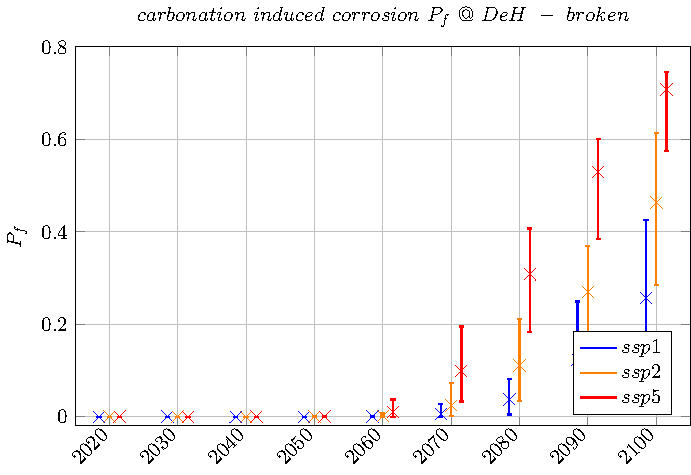
\includegraphics[width=0.8\linewidth]{imgs/pdfs/22_carbonation_comparizon_broken.pdf}
    \caption{Exceedance probabilities comparison between precise and imprecise eBN for carbonation-induced corrosion node and scenarios when the \textit{DeH} is failed}\label{comparizon_carb}
\end{figure}

\begin{figure}[H]
    \centering
    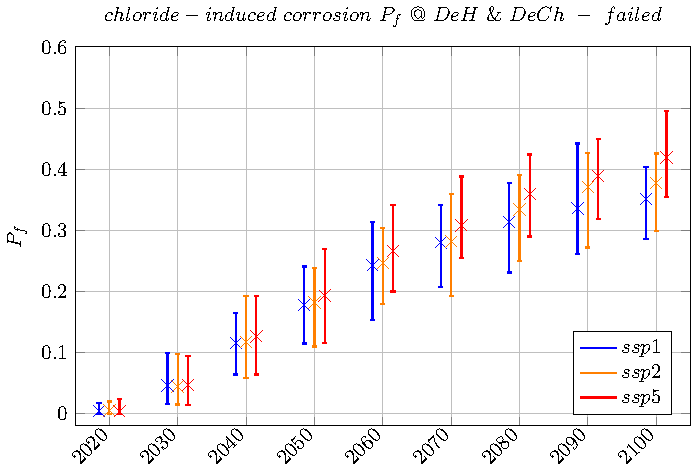
\includegraphics[width=0.8\linewidth]{imgs/pdfs/20_Chloride_comparizon_brokenbroken.pdf}
    \caption{Exceedance probabilities comparison between precise and imprecise eBN for chloride-induced corrosion node and scenarios when both \textit{DeH} and \textit{DeCh} are failed}\label{comparizon_ch_brokenbroken}
\end{figure}

\begin{figure}[H]
    \centering
    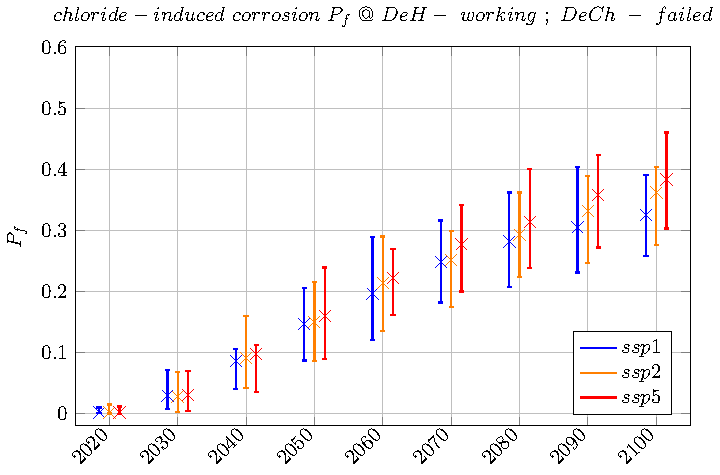
\includegraphics[width=0.8\linewidth]{imgs/pdfs/21_Chloride_comparizon_workingbroken.pdf}
    \caption{Exceedance probabilities comparison between precise and imprecise eBN for chloride-induced corrosion node and scenarios when \textit{DeH} is working and \textit{DeCh} is failed}\label{comparizon_ch_brokenworking}
\end{figure}

    % \subsection{Sensitivity Analysis of Concrete Corrosion Models}
    % \subsection{Exceedance Probabilities for Corrosion}
\section{Conclusions}\label{conclusions}
    Traditional performance assessment of radioactive waste disposals has relied mainly on deterministic framework, based on conservative assumptions. These do not explicitly account for the many uncertainties that affect the assessment. 
In this work, we have developed a framework of imprecise eBN to model concrete corrosion considering epistemic and aleatoric uncertainties, including those stemming from climatic change projections, with a focus on concrete integrity as the primary factor influencing the structural reliability of long-term containment.\\
The adoption of imprecise eBNs enables the aggregation of scenario results within a framework that supports exact-inference algorithms to perform prognostic analysis, for informing decision-making for risk management. Through the use of imprecise probabilities, the framework allows explicitly addressing epistemic uncertainty due to sparse or incomplete data.\\
Although this study has focused on a specific yet critical aspect of radioactive waste disposal performance assessment, namely, the chemical degradation of concrete, the proposed framework is inherently modular and extensible. It can readily accommodate additional degradation mechanisms or coupled physical processes, enabling a more comprehensive safety assessment. Ultimately, such a generalized and uncertainty-aware approach has the potential to complement traditional deterministic frameworks in support of licensing decisions for radioactive waste repositories.\\
The concrete chemical degradation has been described using two models for carbonation-induced and chloride-induced corrosion, showing coherent results in that the failure probabilities consistently fall within the bounds defined by the imprecise intervals.

Despite its advantages, the eBN framework presents certain limitations on the computational side. In fact, precise eBN relies on Monte Carlo simulation for functional node evaluation, which leads to high computational costs. This computational burden is even more exacerbated in the imprecise case due to the need for nested simulations and global optimization, as seen in the Double Loop Monte Carlo and Random Slicing methods.
Future developments should consider incorporating additional degradation phenomena to enrich the risk assessment scope. A unified modelling node for the combined effects of carbonation and chloride-induced corrosion could also be considered, avoiding oversimplified strategies such as logical \textit{OR-gate} or additive approaches, which respectively under- or overestimate the risks. Moreover, optimization of control nodes for parameters like chloride concentration and relative humidity should be undertaken with respect to operational costs and performance. Finally, alternative approximate inference strategies, such as Non Intrusive Stochastic Simulation (NISS)~\cite{wei_non-intrusive_2019} and Collaborative and Adaptive Bayesian Optimization (CABO)~\cite{hong_sequential_2024}, merit investigation to alleviate the computational demand of the imprecise eBN framework.
\newpage

\appendix
    %chktex-file 46
%chktex-file 21
%chktex-file 3
%chktex-file 13
%chktex-file 8
%chktex-file 25
\section{Appendix}\label{appendixA}

To simulate long-term climate behaviour, a range of Global Climate Models (GCMs) is utilized to represent large-scale environmental dynamics. For regional-scale applications, these coarse-resolution outputs are refined through down-scaling techniques using Regional Climate Models (RCMs). Climate projections for Belgium, based on \textit{ssp} scenarios, are derived from the Coupled Model Intercomparison Project Phase 6 (CMIP6), which aggregates output from multiple GCMs and RCMs~\cite{CMIP6,Copernicus_Climate_Change}.\\
The conditional probability tables (CPTs) for temperature, relative humidity, and $CO_2$ concentration nodes in the eBN shown in Fig.~\ref{fig:precise_ebn} are detailed in Tab.~\ref{Climate_Change_Tnode_dists},~\ref{Climate_Change_RHnode_dists}, and~\ref{Climate_Change_CO2node_dists}, respectively. These distributions are estimated by fitting normal distributions at each time step and for each projection.
\begin{table}[H]
    \begin{center}
    \caption{Temperature nodes CPTs for the precise eBN of Fig.\ref{fig:precise_ebn}. Temperatures are measured in $K$}\label{Climate_Change_Tnode_dists}
        \begin{tabular}{P{2.5cm}P{8cm}}
            \toprule
            \textbf{Node} & \textbf{CPT} \\
            \midrule
            $T \_ 2020$ & 
                \begin{tabular}{P{2cm}P{5cm}}
                    \textbf{proj} & \textbf{distribution} \\
                    \midrule
                    \:ssp1 & $Trunc(N(283.9; 0.85); 0, \infty)$ \\
                    \:ssp2 & $Trunc(N(284.1; 0.85); 0, \infty)$ \\
                    \:ssp5 & $Trunc(N(283.9; 0.85); 0, \infty)$ \\
                \end{tabular}
            \\
            \midrule
            $T \_ 2030$ & 
                \begin{tabular}{P{2cm}P{5cm}}
                    \textbf{proj} & \textbf{distribution} \\
                    \midrule
                    \:ssp1 & $Trunc(N(284.2; 0.85); 0, \infty)$ \\
                    \:ssp2 & $Trunc(N(284.2; 0.85); 0, \infty)$ \\
                    \:ssp5 & $Trunc(N(284.3; 1.13); 0, \infty)$ \\
                \end{tabular}
            \\
            \midrule
            $T \_ 2040$ & 
                \begin{tabular}{P{2cm}P{5cm}}
                    \textbf{proj} & \textbf{distribution} \\
                    \midrule
                    \:ssp1 & $Trunc(N(284.2; 0.85); 0, \infty)$ \\
                    \:ssp2 & $Trunc(N(284.6; 0.85); 0, \infty)$ \\
                    \:ssp5 & $Trunc(N(284.9; 1.14); 0, \infty)$ \\
                \end{tabular}
            \\
            \midrule
            $T \_ 2050$ & 
                \begin{tabular}{P{2cm}P{5cm}}
                    \textbf{proj} & \textbf{distribution} \\
                    \midrule
                    \:ssp1 & $Trunc(N(284.5; 0.85); 0, \infty)$ \\
                    \:ssp2 & $Trunc(N(284.8; 1.14); 0, \infty)$ \\
                    \:ssp5 & $Trunc(N(285.4; 1.14); 0, \infty)$ \\
                \end{tabular}
            \\
            \midrule
            $T \_ 2060$ & 
                \begin{tabular}{P{2cm}P{5cm}}
                    \textbf{proj} & \textbf{distribution} \\
                    \midrule
                    \:ssp1 & $Trunc(N(284.7; 1.13); 0, \infty)$ \\
                    \:ssp2 & $Trunc(N(285.1; 0.85); 0, \infty)$ \\
                    \:ssp5 & $Trunc(N(285.9; 1.14); 0, \infty)$ \\
                \end{tabular}
            \\
            \midrule
            $T \_ 2070$ & 
                \begin{tabular}{P{2cm}P{5cm}}
                    \textbf{proj} & \textbf{distribution} \\
                    \midrule
                    \:ssp1 & $Trunc(N(284.7; 1.13); 0, \infty)$ \\
                    \:ssp2 & $Trunc(N(285.2; 1.14); 0, \infty)$ \\
                    \:ssp5 & $Trunc(N(286.5; 1.15); 0, \infty)$ \\
                \end{tabular}
            \\
            \midrule
            $T \_ 2080$ & 
                \begin{tabular}{P{2cm}P{5cm}}
                    \textbf{proj} & \textbf{distribution} \\
                    \midrule
                    \:ssp1 & $Trunc(N(285.0; 1.14); 0, \infty)$ \\
                    \:ssp2 & $Trunc(N(285.4; 1.14); 0, \infty)$ \\
                    \:ssp5 & $Trunc(N(287.4; 1.44); 0, \infty)$ \\
                \end{tabular}
            \\
            \midrule
            $T \_ 2090$ & 
                \begin{tabular}{P{2cm}P{5cm}}
                    \textbf{proj} & \textbf{distribution} \\
                    \midrule
                    \:ssp1 & $Trunc(N(284.8; 1.42); 0, \infty)$ \\
                    \:ssp2 & $Trunc(N(286.7; 1.14); 0, \infty)$ \\
                    \:ssp5 & $Trunc(N(288.1; 1.44); 0, \infty)$ \\
                \end{tabular}
            \\
            \midrule
            $T \_ 2100$ & 
                \begin{tabular}{P{2cm}P{5cm}}
                    \textbf{proj} & \textbf{distribution} \\
                    \midrule
                    \:ssp1 & $Trunc(N(283.7; 1.42); 0, \infty)$ \\
                    \:ssp2 & $Trunc(N(286.0; 1.14); 0, \infty)$ \\
                    \:ssp5 & $Trunc(N(288.9; 1.45); 0, \infty)$ \\
                \end{tabular}
        \end{tabular}
    \end{center}
\end{table}

\begin{table}[H]
    \begin{center}
        \caption{RH nodes CPTs for the precise eBN of Fig.\ref{fig:precise_ebn}. RH is expressed in percentage of deviation wth respect to the reference value $RH_{ref}$ = 0.65}\label{Climate_Change_RHnode_dists}
        \begin{tabular}{P{2.5cm}P{8cm}}
            \toprule
            \textbf{Node} & \textbf{CPT} \\
            \midrule
            $RH \_ int \_ 2020$ & 
                \begin{tabular}{P{2cm}P{5cm}}
                    \textbf{proj} & \textbf{distribution} \\
                    \midrule
                    \:ssp1 & $Trunc(N(9.35e^{-2}; 5.66e^{-2}); 0, 1)$ \\
                    \:ssp2 & $Trunc(N(8.48e^{-2}; 6.42e^{-2}); 0, 1)$ \\
                    \:ssp5 & $Trunc(N(8.19e^{-2}; 5.00e^{-2}); 0, 1)$ \\
                \end{tabular}
            \\
            \midrule
            $RH \_ int \_ 2030$ & 
                \begin{tabular}{P{2cm}P{5cm}}
                    \textbf{proj} & \textbf{distribution} \\
                    \midrule
                    \:ssp1 & $Trunc(N(9.52e^{-2}; 5.20e^{-2}); 0, 1)$ \\
                    \:ssp2 & $Trunc(N(9.18e^{-2}; 5.42e^{-2}); 0, 1)$ \\
                    \:ssp5 & $Trunc(N(1.11e^{-1}; 5.83e^{-2}); 0, 1)$ \\
                \end{tabular}
            \\
            \midrule
            $RH \_ int \_ 2040$ & 
                \begin{tabular}{P{2cm}P{5cm}}
                    \textbf{proj} & \textbf{distribution} \\
                    \midrule
                    \:ssp1 & $Trunc(N(1.01e^{-1}; 5.67e^{-2}); 0, 1)$ \\
                    \:ssp2 & $Trunc(N(1.12e^{-1}; 6.61e^{-2}); 0, 1)$ \\
                    \:ssp5 & $Trunc(N(1.44e^{-1}; 7.07e^{-2}); 0, 1)$ \\
                \end{tabular}
            \\
            \midrule
            $RH \_ int \_ 2050$ & 
                \begin{tabular}{P{2cm}P{5cm}}
                    \textbf{proj} & \textbf{distribution} \\
                    \midrule
                    \:ssp1 & $Trunc(N(1.16e^{-1}; 6.56e^{-2}); 0, 1)$ \\
                    \:ssp2 & $Trunc(N(1.34e^{-1}; 6.63e^{-2}); 0, 1)$ \\
                    \:ssp5 & $Trunc(N(1.66e^{-1}; 6.73e^{-2}); 0, 1)$ \\
                \end{tabular}
            \\
            \midrule
            $RH \_ int \_ 2060$ & 
                \begin{tabular}{P{2cm}P{5cm}}
                    \textbf{proj} & \textbf{distribution} \\
                    \midrule
                    \:ssp1 & $Trunc(N(1.27e^{-1}; 6.63e^{-2}); 0, 1)$ \\
                    \:ssp2 & $Trunc(N(1.50e^{-1}; 7.39e^{-2}); 0, 1)$ \\
                    \:ssp5 & $Trunc(N(1.90e^{-1}; 7.26e^{-2}); 0, 1)$ \\
                \end{tabular}
            \\
            \midrule
            $RH \_ int \_ 2070$ & 
                \begin{tabular}{P{2cm}P{5cm}}
                    \textbf{proj} & \textbf{distribution} \\
                    \midrule
                    \:ssp1 & $Trunc(N(1.25e^{-1}; 6.80e^{-2}); 0, 1)$ \\
                    \:ssp2 & $Trunc(N(1.60e^{-1}; 8.14e^{-2}); 0, 1)$ \\
                    \:ssp5 & $Trunc(N(2.30e^{-1}; 8.92e^{-2}); 0, 1)$ \\   
                \end{tabular}
            \\
            \midrule
            $RH \_ int \_ 2080$ & 
                \begin{tabular}{P{2cm}P{5cm}}
                    \textbf{proj} & \textbf{distribution} \\
                    \midrule
                    \:ssp1 & $Trunc(N(1.42e^{-1}; 7.54e^{-2}); 0, 1)$ \\
                    \:ssp2 & $Trunc(N(1.71e^{-1}; 7.88e^{-2}); 0, 1)$ \\
                    \:ssp5 & $Trunc(N(2.95e^{-1}; 1.91e^{-1}); 0, 1)$ \\   
                \end{tabular}
            \\
            \midrule
            $RH \_ int \_ 2090$ & 
                \begin{tabular}{P{2cm}P{5cm}}
                    \textbf{proj} & \textbf{distribution} \\
                    \midrule
                    \:ssp1 & $Trunc(N(1.41e^{-1}; 8.12e^{-2}); 0, 1)$ \\
                    \:ssp2 & $Trunc(N(1.79e^{-1}; 8.25e^{-2}); 0, 1)$ \\
                    \:ssp5 & $Trunc(N(3.28e^{-1}; 1.24e^{-1}); 0, 1)$ \\
                \end{tabular}
            \\
            \midrule
            $RH \_ int \_ 2100$ & 
                \begin{tabular}{P{2cm}P{5cm}}
                    \textbf{proj} & \textbf{distribution} \\
                    \midrule
                    \:ssp1 & $Trunc(N(1.34e^{-1}; 8.97e^{-2}); 0, 1)$ \\
                    \:ssp2 & $Trunc(N(1.96e^{-1}; 8.64e^{-2}); 0, 1)$ \\
                    \:ssp5 & $Trunc(N(3.85e^{-1}; 1.43e^{-1}); 0, 1)$ \\
                \end{tabular}
        \end{tabular}
    \end{center}
\end{table}

\begin{table}[H]
    \begin{center}
    \caption{$CO_2$ concentration nodes CPTs for the precise eBN of Fig.\ref{fig:precise_ebn}. $CO_2$ concentrations are measured in $ppm$}\label{Climate_Change_CO2node_dists}
        \begin{tabular}{P{2.7cm}P{8cm}}
            \toprule
            \textbf{Node} & \textbf{CPT} \\
            \midrule
            $ppm \_CO_2 \_ 2020$ & 
                \begin{tabular}{P{2cm}P{5cm}}
                    \textbf{proj} & \textbf{distribution} \\
                    \midrule
                    \:ssp1 & $412.5$ \\
                    \:ssp2 & $412.5$ \\
                    \:ssp5 & $412.5$ \\
                \end{tabular}
            \\
            \midrule
            $ppm \_CO_2 \_ 2030$ & 
                \begin{tabular}{P{2cm}P{5cm}}
                    \textbf{proj} & \textbf{distribution} \\
                    \midrule
                    \:ssp1 & $Trunc(N(430.8; 6.89); 0)$ \\
                    \:ssp2 & $Trunc(N(435.0; 7.83); 0)$ \\
                    \:ssp5 & $Trunc(N(448.8; 9.87); 0)$ \\
                \end{tabular}
            \\
            \midrule
            $ppm \_CO_2 \_ 2040$ & 
                \begin{tabular}{P{2cm}P{5cm}}
                    \textbf{proj} & \textbf{distribution} \\
                    \midrule
                    \:ssp1 & $Trunc(N(440.2; 6.89); 0)$ \\
                    \:ssp2 & $Trunc(N(460.8; 7.37); 0)$ \\
                    \:ssp5 & $Trunc(N(489.4; 8.80); 0)$ \\
                \end{tabular}
            \\
            \midrule
            $ppm \_CO_2 \_ 2050$ & 
                \begin{tabular}{P{2cm}P{5cm}}
                    \textbf{proj} & \textbf{distribution} \\
                    \midrule
                    \:ssp1 & $Trunc(N(442.7; 7.52); 0)$ \\
                    \:ssp2 & $Trunc(N(486.5; 7.30); 0)$ \\
                    \:ssp5 & $Trunc(N(540.5; 10.27); 0)$ \\
                \end{tabular}
            \\
            \midrule
            $ppm \_CO_2 \_ 2060$ & 
                \begin{tabular}{P{2cm}P{5cm}}
                    \textbf{proj} & \textbf{distribution} \\
                    \midrule
                    \:ssp1 & $Trunc(N(441.7; 4.41); 0)$ \\
                    \:ssp2 & $Trunc(N(508.9; 8.14); 0)$ \\
                    \:ssp5 & $Trunc(N(603.5; 9.05); 0)$ \\
                \end{tabular}
            \\
            \midrule
            $ppm \_CO_2 \_ 2070$ & 
                \begin{tabular}{P{2cm}P{5cm}}
                    \textbf{proj} & \textbf{distribution} \\
                    \midrule
                    \:ssp1 & $Trunc(N(437.5; 3.50); 0)$ \\
                    \:ssp2 & $Trunc(N(524.3; 7.34); 0)$ \\
                    \:ssp5 & $Trunc(N(677.1; 8.80); 0)$ \\
                \end{tabular}
            \\
            \midrule
            $ppm \_CO_2 \_ 2080$ & 
                \begin{tabular}{P{2cm}P{5cm}}
                    \textbf{proj} & \textbf{distribution} \\
                    \midrule
                    \:ssp1 & $Trunc(N(431.6; 3.88); 0)$ \\
                    \:ssp2 & $Trunc(N(531.1; 6.37); 0)$ \\
                    \:ssp5 & $Trunc(N(758.2; 9.86); 0)$ \\
                \end{tabular}
            \\
            \midrule
            $ppm \_CO_2 \_ 2090$ & 
                \begin{tabular}{P{2cm}P{5cm}}
                    \textbf{proj} & \textbf{distribution} \\
                    \midrule
                    \:ssp1 & $Trunc(N(426.0; 4.26); 0)$ \\
                    \:ssp2 & $Trunc(N(533.7; 5.34); 0)$ \\
                    \:ssp5 & $Trunc(N(844.8; 10.13); 0)$ \\
                \end{tabular}
            \\
            \midrule
            $ppm \_CO_2 \_ 2100$ & 
                \begin{tabular}{P{2cm}P{5cm}}
                    \textbf{proj} & \textbf{distribution} \\
                    \midrule
                    \:ssp1 & $Trunc(N(420.9; 4.63); 0)$ \\
                    \:ssp2 & $Trunc(N(538.4; 4.30); 0)$ \\
                    \:ssp5 & $Trunc(N(935.9; 9.36); 0)$ \\
                \end{tabular}
        \end{tabular}
    \end{center}
\end{table}


\section{Appendix}\label{appendixB}
The same data set used for Appendix~\ref{appendixA} have been employed to build the intervals for each temperature node of the imprecise eBN shown in Fig.~\ref{fig:imprecise_ebn}. Lower and upper interval bounds have been evaluated respectively as the 95\% lower and upper confidence intervals.
\begin{table}[H]
    \begin{center}
    \caption{Temperature nodes CPTs for the imprecise eBN of Fig.\ref{fig:imprecise_ebn}. Temperatures are measured in $K$}\label{Climate_Change_Tnode_interval}
        \begin{tabular}{P{2.5cm}P{7.7cm}}
            \toprule
            \textbf{Node} & \textbf{CPT} \\
            \midrule
            $T \_ 2020$ & 
                \begin{tabular}{P{2.4cm}P{2cm}P{2cm}}
                    \textbf{proj} & \textbf{lb} & \textbf{ub}\\
                    \midrule
                    \:ssp1 & $281.8723$ & $285.5608$\\ 
                    \:ssp2 & $281.6916$ & $286.8414$ \\
                    \:ssp5 & $281.5062$ & $286.7255$ \\
                \end{tabular}
            \\
            \midrule
            $T \_ 2030$ & 
                \begin{tabular}{P{2.4cm}P{2cm}P{2cm}}
                    \textbf{proj} & \textbf{lb} & \textbf{ub}\\
                    \midrule
                    \:ssp1 & $282.0982$ & $287.0741$ \\
                    \:ssp2 & $282.2602$ & $286.8415$ \\
                    \:ssp5 & $281.5062$ & $286.7255$ \\
                \end{tabular}
            \\
            \midrule
            $T \_ 2040$ & 
                \begin{tabular}{P{2.4cm}P{2cm}P{2cm}}
                    \textbf{proj} & \textbf{lb} & \textbf{ub}\\
                    \midrule
                    \:ssp1 & $282.2752$ & $285.7549$ \\
                    \:ssp2 & $282.2368$ & $287.6774$ \\
                    \:ssp5 & $281.8712$ & $287.1479$ \\
                \end{tabular}
            \\
            \midrule
            $T \_ 2050$ & 
                \begin{tabular}{P{2.4cm}P{2cm}P{2cm}}
                    \textbf{proj} & \textbf{lb} & \textbf{ub}\\
                    \midrule
                    \:ssp1 & $282.1972$ & $286.3009$ \\
                    \:ssp2 & $282.1169$ & $286.5602$ \\
                    \:ssp5 & $282.6306$ & $287.7634$ \\
                \end{tabular}
            \\
            \midrule
            $T \_ 2060$ & 
                \begin{tabular}{P{2.4cm}P{2cm}P{2cm}}
                    \textbf{proj} & \textbf{lb} & \textbf{ub}\\
                    \midrule
                    \:ssp1 & $281.9507$ & $287.6729$ \\
                    \:ssp2 & $282.8809$ & $287.8323$ \\
                    \:ssp5 & $284.1444$ & $288.1458$ \\
                \end{tabular}
            \\
            \midrule
            $T \_ 2070$ & 
                \begin{tabular}{P{2.4cm}P{2cm}P{2cm}}
                    \textbf{proj} & \textbf{lb} & \textbf{ub}\\
                    \midrule
                    \:ssp1 & $282.4679$ & $286.3140$ \\
                    \:ssp2 & $282.1799$ & $287.8909$ \\
                    \:ssp5 & $283.5394$ & $289.1019$ \\
                \end{tabular}
            \\
            \midrule
            $T \_ 2080$ & 
                \begin{tabular}{P{2.4cm}P{2cm}P{2cm}}
                    \textbf{proj} & \textbf{lb} & \textbf{ub}\\
                    \midrule
                    \:ssp1 & $282.0230$ & $287.2399$ \\
                    \:ssp2 & $283.1048$ & $287.3655$ \\
                    \:ssp5 & $284.8888$ & $289.7104$ \\
                \end{tabular}
            \\
            \midrule
            $T \_ 2090$ & 
                \begin{tabular}{P{2.4cm}P{2cm}P{2cm}}
                    \textbf{proj} & \textbf{lb} & \textbf{ub}\\
                    \midrule
                    \:ssp1 & $281.3064$ & $288.7765$ \\
                    \:ssp2 & $282.5490$ & $287.8518$ \\
                    \:ssp5 & $284.3658$ & $290.5262$ \\
                \end{tabular}
            \\
            \midrule
            $T \_ 2100$ & 
                \begin{tabular}{P{2.4cm}P{2cm}P{2cm}}
                    \textbf{proj} & \textbf{lb} & \textbf{ub}\\
                    \midrule
                    \:ssp1 & $281.7551$ & $287.4349$ \\
                    \:ssp2 & $283.0796$ & $288.4324$ \\
                    \:ssp5 & $285.1481$ & $292.2743$ \\
                \end{tabular}
        \end{tabular}
    \end{center}
\end{table}

\newpage

\printbibliography{}
\end{document}